
% ----------------------------------------------------------------------
%                   LATEX TEMPLATE FOR PhD THESIS
% ----------------------------------------------------------------------

% based on Harish Bhanderi's PhD/MPhil template, then Uni Cambridge
% http://www-h.eng.cam.ac.uk/help/tpl/textprocessing/ThesisStyle/
\documentclass[twoside,11pt]{Latex/Classes/PhDthesisPSnPDF}
% This file contains macros that can be called up from connected TeX files
% It helps to summarise repeated code, e.g. figure insertion (see below).


\renewcommand{\baselinestretch}{2.5}

% for four node types
\def\Nc#1#2{\hbox{\texttt{#1$_{#2}$}}}
\def\Nl#1#2{\hbox{$\bullet$\texttt{#1$_{#2}$}}}
\def\Nr#1#2{\hbox{\texttt{#1$_{#2}$}$\bullet$}}
\def\Np#1#2{\hbox{$\bullet$\texttt{#1$_{#2}$}$\bullet$}}

\def\PT#1{\hbox{\textrm{pt}$_{#1}$}}
\def\pred#1#2{#1\to\{#2\}}
\def\INDEXSET#1{\mathit{#1}_{[P]}}
\def\INDEXSETL#1{\mathit{#1}_{[p]}}

\newtheorem{property}{Property}


% uncomment to print only "1" not "Chapter 1"
%\renewcommand{\chaptername}{}

% insert a centered figure with caption and description
% parameters 1:filename, 2:title, 3:description and label
\newcommand{\figuremacro}[3]{
	\begin{figure}[htbp]
		\centering
		\includegraphics[width=1\textwidth]{#1}
		\caption[#2]{\textbf{#2} - #3}
		\label{#1}
	\end{figure}
}

% insert a centered figure with caption and description AND WIDTH
% parameters 1:filename, 2:title, 3:description and label, 4: textwidth
% textwidth 1 means as text, 0.5 means half the width of the text
\newcommand{\figuremacroW}[4]{
	\begin{figure}[htbp]
		\centering
		\includegraphics[width=#4\textwidth]{#1}
		\caption[#2]{\textbf{#2} - #3}
		\label{#1}
	\end{figure}
}

% inserts a figure with wrapped around text; only suitable for NARROW figs
% o is for outside on a double paged document; others: l, r, i(inside)
% text and figure will each be half of the document width
% note: long captions often crash with adjacent content; take care
% in general: above 2 macro produce more reliable layout
\newcommand{\figuremacroN}[3]{
	\begin{wrapfigure}{o}{0.5\textwidth}
		\centering
		\includegraphics[width=0.48\textwidth]{#1}
		\caption[#2]{{\small\textbf{#2} - #3}}
		\label{#1}
	\end{wrapfigure}
}

% predefined commands by Harish
\newcommand{\PdfPsText}[2]{
  \ifpdf
     #1
  \else
     #2
  \fi
}

\newcommand{\IncludeGraphicsH}[3]{
  \PdfPsText{\includegraphics[height=#2]{#1}}{\includegraphics[bb = #3, height=#2]{#1}}
}

\newcommand{\IncludeGraphicsW}[3]{
  \PdfPsText{\includegraphics[width=#2]{#1}}{\includegraphics[bb = #3, width=#2]{#1}}
}

\newcommand{\InsertFig}[3]{
  \begin{figure}[!htbp]
    \begin{center}
      \leavevmode
      #1
      \caption{#2}
      \label{#3}
    \end{center}
  \end{figure}
}




%: ----------------------------------------------------------------------
%:                  TITLE PAGE: name, degree,..
% ----------------------------------------------------------------------
% below is to generate the title page with crest and author name

%if output to PDF then put the following in PDF header
\ifpdf
    \pdfinfo { /Title  (PhD and MPhil Thesis Classes)
               /Creator (LaTeX)
               /Producer ()
               /Author (Wei HAO your@email.net)
               /CreationDate (D:YYYYMMDDhhmmss)  %format D:YYYYMMDDhhmmss
               /ModDate (D:YYYYMMDDhhmm)
               /Subject (xyz)
               /Keywords (add, your, keywords, here) }
    \pdfcatalog { /PageMode (/UseOutlines)
                  /OpenAction (fitbh)  }
\fi


\title{A Study on Large XML Processing, Fragmentation, Query and XPath processing}


% ----------------------------------------------------------------------
% The section below defines www links/email for author and institutions
% They will appear on the title page of the PDF and can be clicked
\ifpdf
  \author{\href{mailto:your@email.net}{Wei HAO}}
  \cityofbirth{born in Huainan, Anhui, China}

  \collegeordept{\href{http://www.something.net}{Informatics of Computer Science}}
  \university{\href{http://www.something.net}{Kochi University of Technology}}
  \crest{
\includegraphics[width=4cm]{frontmatter/figures/logo}}
% If you are not creating a PDF then use the following. The default is PDF.
\else
  \author{YourName}
  \cityofbirth{born in Huainan, Anhui, China}
  \collegeordept{CollegeOrDept}
  \university{University}
  \crest{
\includegraphics[width=4cm]{logo}}
\fi

%\renewcommand{\submittedtext}{change the default text here if needed}
\degree{Doctor of Philosophy}
\degreedate{September 2017}


% ----------------------------------------------------------------------
% turn of those nasty overfull and underfull hboxes
\hbadness=10000
\hfuzz=50pt


%: --------------------------------------------------------------
%:                  FRONT MATTER: dedications, abstract,..
% --------------------------------------------------------------

\begin{document}

% sets line spacing
\renewcommand\baselinestretch{1.2}
\baselineskip=18pt plus1pt


%: ----------------------- generate cover page ------------------------

\maketitle  % command to print the title page with above variables

\mainmatter
\renewcommand{\chaptername}{} % uncomment to print only "1" not "Chapter 1"

% The introduction of the thesis.

\chapter{Introduction}

\section{Background}

In recent decades, the volume of information increases dramatically, leading to
an urgent demand for high-performance data processing technologies, as well as
in the field of large XML document processing.  XML document processing as a
common and popularly used information processing technique and has been
intensively studied. The sizes of XML documents are also increasing
dramatically. For example,  Wikipedia~\cite{wiki} provides a dump
service~\cite{wikipediadump} that exports wikitext source and metadata embedded
in XML documents. The sizes of the data was less than one gigabyte before 2006.
In just 10 years, it increased to over 100 gigabytes nowadays~\cite{wikisize}.
Some XML documents even reach hundreds of gigabyte. For example, an online
database of protein sequence UniProtKB~\cite{UniProtKB} can store all the data
in a single XML document sized 358 GB.

Up to the beginning of this century, studies of XML processing mainly  focused
on sequential processing~\cite{Skil97,AlJYK02,Ne02,ToGr02,HAJR03},  due to that
commonly used CPUs were mostly single-core processors. As the multiple-core CPUs
gradually became dominant gradually,  more researches shifted to parallel XML
processing  and thus more related studies were
proposed~\cite{SAFu05,PaZC08,LFLQ08,ZhPC10}.

One common topic in the field of parallel XML processing is the parallelization
of XPath~\cite{xpath} queries over XML documents. The basic idea of parallelize
is to divide an XML document into multiple parts and process queries separately
in parallel. One key problem of the parallelization is how to deal with the
hierarchical structure that is the intrinsic characteristic of each XML
document. This characteristic plays a very important role in parallel XML
document processing, forcing us to deal with the connections of the divided
parts after splitting. 

To address the above difficulty, many approaches had been proposed~\cite{JLWO03,
SAFu05,NEMH07,BuLM08,Mats09, ZhPC10,ChLW13,HaMa16}. Most of these approaches
tend to represent XML document as trees and preserve them in memory, then
parallelizing XML processing on these trees, which usually utilize multi-thread
techniques processed in a shared memory where all the threads are able to access
the shared XML data. However, these studies discuss the parallelization of XPath
queries only on the a whole tree (or a number of whole trees) without
considering how to divide them. Thus, they are not suitable for distribued XML
document processing.

Another common approach of XML processing is to exploit database techniques. XML
processing in databases has also been widely
studied~\cite{fong2001converting,meier2002exist,jagadish2002timber,jiang2002xparent,PCSS04}.
Common database techniques, such as
indexing~\cite{kha2001xml,wang2005sequencing,popovici2005sirius}, join
algorithms~\cite{liang2005lax,liang2006slax,guha2003index}, are also valid to be
applied to XML processing. Although the concurrent transactions are available in
modern database engines, making it possible and available to be used  in
distribued settings,  there is, to the best of our knowledge, no existing work
that focuses on the parallelization of XPath queries in XML databases.
Therefore, to parallelize the evaluation of XPath queries in XML databases, we
address the following two challenges.

\begin{itemize} \item Parallelizing Evaluation of A Single XPath Query. \\ By
dividing or rewriting an XPath queries into multiple subqueries, such
as~\cite{BoLS09,Bord10},  we can convert the evaluation of the original query to
the evaluation of these subqueries. However, it is a technical difficulty to
figure out how to parallelize the evaluation of an single query by exploiting
existing XML database engines, particularly how to achieve good performance gain
and scalability.

\item Parallelizing Evaluation of queries in distributed-memory environments.\\
When processing XML documents in distributed-memory environments, it is common
to partition an XML document into chunks and distribute the processing of chunk
to multiple computers. However, how to represent chunks and evaluate queries on
them for efficient evaluation, and how to handle the communication among
computers are still challenges for efficient XML processing. \end{itemize}

This thesis addresses the above problems and there are two approaches proposed
for both shared-memory environments and distributed-memory environments,
particularly for the latter. In the following section, we present a ``short
tour'' to illustrate the contributions of this thesis.

\section{A Short Tour}

To address the parallelization of XPath queries in XML databases, we demonstrate
our two approaches with examples.

The first approach involves an implmentation work of~\cite{BoLS09} proposed by
Bordawekar et al., which presented approaches to easily exploit esxisting XML
processors, such as Xalan~\cite{xalan}, to parallelize XPath queires with no
need to modify  the processors. Their approach was to partition queries in an ad
hoc manner and to merge the results of partitioned queries. Specifically, they
proposed three strategies: query partitioning, data partitioning and hybrid
partitioning. Query partitioning is to split a given query into independent
queries by using predicates, e.g., from \texttt{$q_1$[$q_2$ or $q_3$]} to
\texttt{$q_1$[$q_2$]} and \texttt{$q_1$[$q_3$]}, and from \texttt{$q_1$/$q_2$}
to \texttt{$q_1$[position() <= n]/$q_2$} and \texttt{$q_1$[position() >
n]/$q_2$}. Data partitioning is to split a given query into a prefix query and a
suffix query, e.g., from \texttt{$q_1$/$q_2$} to prefix $q_1$ and suffix $q_2$,
and to run the suffix query in parallel on each node of the result of the prefix
query. How to merge depends on the partitioning strategies.  Since hybrid
partitioning strategy is a mix of the first two partitioning strategies, we
focus on the data partitioning and query partitioning strategies in this thesis.
For query partitioning, it depends on the relationships of subqueries in the
predicate. If we split and-/or-predicates, we have to intersect/union results.
For data partitioning, if we perform position-based query partitioning and data
partitioning, we have only to concatenate results in order. In our study, we
have developed two implementations of data-partitioning parallelization and a
implementation of query-partitioning parallelization on top of
BaseX~\cite{basex864}, which is a state-of-the-art XML database engine.

The second approach is based on a novel tree structure, called partial tree. A
partital tree is a tree strcutre for representing a chunk of an XML document so
that XPath queries can be evaluated on partial trees of an XML documents in
parallel. Partial trees can be use in both shared-memory and distributed-memory
environments. To understand what a partial tree is and how it works, we use the
following XML document as an example.

\begin{quote}\small\tt
<A><B><C>c1</C><C>c\underline{2</C><C>c3</C><A><C>c4</C><B>}\\
</B></A></B><A><B></B></A><B></B></A> \end{quote}

We can construct a tree as shown in Figure~\ref{fig:exampletree} for
representing the given XML document. Note that each node in the tree structure
is formed by parsing a pair of tags, the start tag and the end tag. The tags in
between a pair of tags form nodes as children or descendants of the node formed
by the pair of tags. As we know, a node in the tree structure should come from a
pair of tags, but not a single tag. Thus, here comes a question: \emph{What
structure can a single tag represent in the tree\/}?

For example, consider the underlined part of the document in
Figure~\ref{fig:exampletree}. The corresponding nodes of tags in the underlined
part are colored gray in the figure. Note that some tags, such as the first
\verb|</C>| or the last \verb|<B>| miss their matching tags. Then, how can we
represent these tags when we parse this chunk?  Besides, A$_1$ and B$_2$ are
missing in the chunk. Therefore, how can we apply  queries to the gray part in
the figure in case we do not know the path  from it to the root of the whole
tree, i.e.  A$_1$ and B$_2$?

\begin{figure}[t]
\centering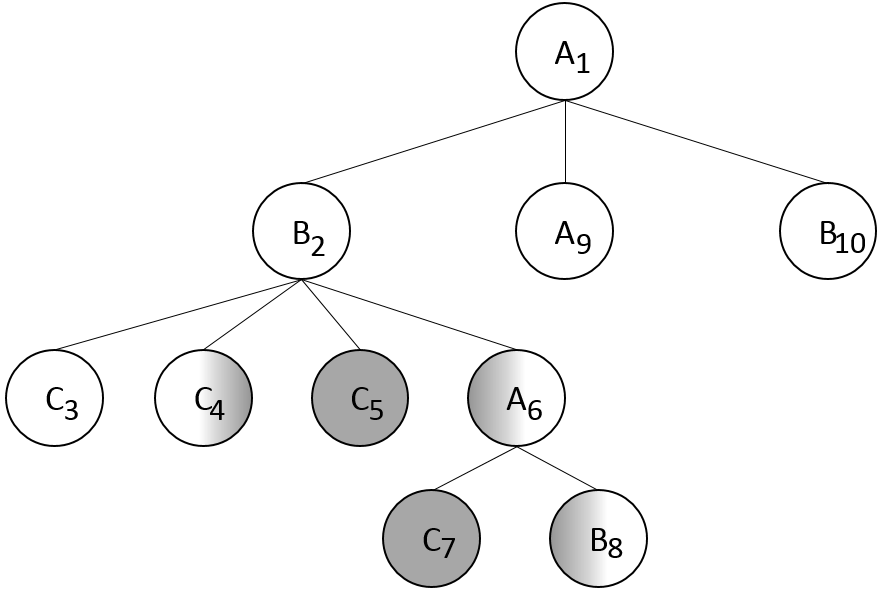
\includegraphics[scale=0.3]{introduction/figures/exampletree.png}
\caption{An example XML tree} \label{fig:exampletree}
\centering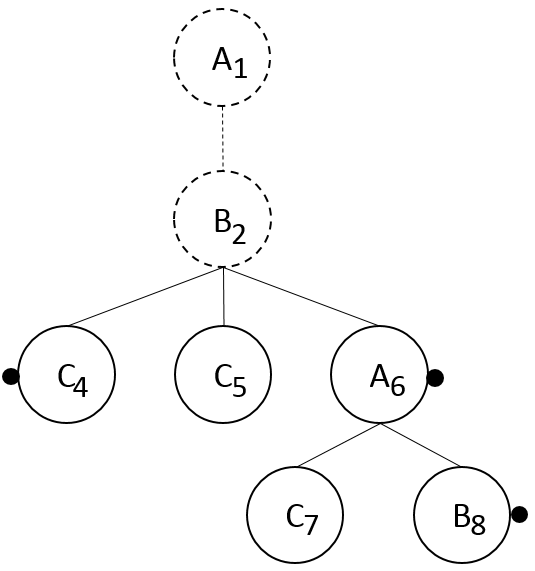
\includegraphics[scale=0.3]{introduction/figures/examplepartialtree.png}
\caption{Partial tree for the example.} \label{fig:examplepartialtree}
\end{figure}

To address on the above two problems, we first proposed a novel tree structure,
called partial tree. As show in Figure 1.2.  We can create a partial tree for
the chunk. The partial tree has the information  of the missing path, i.e. A1
and B2. This tree is different from ordinary trees  because we define some
special nodes for partial tree (These special nodes with  dots in the feature
will be discussed at length in Section~\ref{sec:partialtree}).

By adding the nodes on the path from the root to the current chunk part, we are
now able to apply the queries to this partial tree based on the parent-child
relationships. We will discuss the query algorithms in
Section~\ref{sec:queryalgo}. Although partial tree is available in both
shared-/distributed- memory environments, it is more specially designed for
distributed-memory environments. This is becuase chunks of an XML documents can
distribted to multiple computers and then be parsed into partial trees for
further parallel processing.

\section{Contributions}

We consider three key contributions in the thesis.

The first contribution involves implementations of~\cite{BoLS09}, and our
observations and perspectives from the experiment results. Our implementations
are designed for the parallelization of XPath queries on top of BaseX, which is
a state-of-the-art XML database engine and XPath/XQuery 3.1 processor. With
these implementations, XPath queries can be easily parallelized by simply
rewriting XPath queries with XQuery expressions. We conduct experiments to
evaluate our implementations and the results showed that these implementations
achieved significant speedups over XML documents sized several gigabytes.
Besides the experiment results, we also present significant observations and
perspectives from the experiment results.

The second contribution is the design of a novel tree structure, called partial
tree, for parallel XML processing. With this tree structure, we can split an XML
document into multiple chunks and represent each of the chunks with partial
trees. We also design a series of algorithms for evaluating queries over these
partial trees. Since the partial trees are created from separated chunks, we can
distribute these chunks to computer clusters. In this way, we can run queries on
them in distributed memory environments. We also proposed an efficient
implementation of partial tree. Based on indexing techniques, we developed a
indexing scheme, called BFS-array index along with grouped index. With this
indexing scheme, we can implement partial tree efficiently, in both memory
consumption and absolute query performance. The experiments showed that the
implementation can process 100s GB of XML documents with 32 EC2 computers. The
execution times were only seconds for most queries used in the experiments and
the throughput was approximately 1 GB/s.

\section{Outline}

The thesis is organized in six chapters. An introduction to this study is given
in Chapter 1. We  review the  related work in Chapter 2 and give definitions of
XML query languages in Chapter 3. We propose the idea of XPath queries on top of
BaseX in Chapter 4. We propose the new tree structure, partial tree in Chapter 5
and  we conclude the whole thesis in Chapter 6. Here are the detailed
introduction to the following Chapters.

Chatper 2

We dicuss the related work in three aspects: XML fragmentation, parallel
evaluation of XML queries and XML database techniques.

Chapter 3

In this section, the definitions of XML and two XML query languages, XPath and
XQuery are introduced and defined.

Chapter 4

We introduce our implementations of \cite{BoLS09}.  We introduce the XML
processing engine BaseX and we present our implementations. We evaluate our
implementations on two data sets and propose our observations and perspectives
from the experiment results.

Chapter 5

We present a noval tree structure, partial tree. We give the definitions of
partial tree, discuss the characteristics and design querying algorithms for
partial tree. We also propose an efficient BFS-index based implementation of
partial tree. We report the experiment results and analyze the results.

Chapter 6

We summarize this thesis and discuss the future work.



\chapter{Related Work}
\label{sec:relatedwork}

We discuss related work in three related fields, XML fragmentation, parallel XML
processing and XML database Techniques.

\section{XML Fragmentation}

Fragmentation is an important way of efficient processing XML documents, which
divides an XML document in fragments and processes them in parallel.
Fragmentation is the premise of data-parallel computation algorithms, and has
been intensively
studied~\cite{ARBM06,DaGP14,CFKL12,NEMH07,OgTP13,LiZZ17,CFKL12,DaGP14}. We
discuss three ways of fragmentations of XML documents in this section.

\subsection{Fragmentation of Trees}

Data fragmentation is characterized by physical changes to the dataset, that is,
the dataset is fragmented and allocated to multiple computational
nodes~\cite{BrMa14}. Kling et al.~\cite{kling11:dist_xml} modeled fragmentation
as horizontal and vertical in terms of XML schema~\cite{schema} that is a
language for expressing constraints about XML documents. We now discuss these
two fragmentations.

\subsubsection{Horizontal Fragmentation}
\label{sec:hfragment}

Horizontal fragmentation is to divide a document tree into multiple fragments
and every fragment follows the same schema of the original XML document. The
whole document is a simple collection of fragments. Horizontal fragmentation is
rather straightforward and widely used in parallel XML
processing~\cite{DaGP14,BoLS09,AfDG15,CCMN15}. Since the fragments follow the
same schema, the queries can be evaluated on them by considering the schema.

\subsubsection{Vertical Fragmentation}
\label{sec:vfragment}

Vertical fragmentation, on the other hand, is a fragmentation that extracts
subtrees from the middle of the tree, thus following different schemas. Though
this fragmentation does not usually work well for parallel XML processing, it is
worth studying. This is because it is a possible and  important in case when the
data are integrated from different sites or organizations~\cite{CFKL12,KlOD10}.

\subsection{Fragmentation of XML Text}

Compared to these tree-based fragmentation techniques, the fragmentation in this
study is based on serialized text, which means we cast the partition on the
plain text of an XML document in stead of the XML tree parsed from the document.
The main advantage of our text-based fragmentation is that we can assign the
chunks over distributed file systems~\cite{dfs} that are cut by default. Similar
idea was introduced by Choi et al.~\cite{ChLL14} in which they added labels to
make every chunk a well-formed tree in a preparsing phase.

\subsection{Holes and Fillers}

Bose et al. proposed a fragmentation model~\cite{bose2003query}. Bese on this,
Bose  et al. proposed a system called Xfrag~\cite{bose2005xfrag}. In this
system, an document is divided into multiple sub documents called fillers,
where other fragments (the fillers) may fit.  Cong et al.~\cite{CFKL12} and
Nomura et al. \cite{NEMH07} adopted a tree-shaped fragment that contains
original nodes and hole nodes, where a hole node represents a link to a missing
subtree, and represented the whole document as a tree of fragments. The key part
of their approaches to decouple dependencies between evaluations on fragments so
as to perform them in parallel.


\section{Parallel XML Processing}
\label{sec:paralleleval}

Many existing studies address the topic of XML processing in
parallel~\cite{BoLS09,PaZC08,LuGa08,Mats09,SAFu05}. We discuss parallel XML
processing in this section.

\subsection{Tree Accumulation and Reduction}

There are some exsisting ideas of dividing the XML documents and running the
computation for trees called tree reduction. Kakehi et al.~\cite{KaME07} showed
a parallel tree reduction algorithm from the nodes in chunks. Based on the idea
given by Kakehi et al., Emoto and Imachi~\cite{EmIm12} developed a parallel tree
reduction algorithm on Hadoop, and Matsuzaki and Miyazaki~\cite{MaMi16}
developed a parallel tree accumulation algorithm. A similar approach was taken
by Sevilgen et al.~\cite{SAFu05} who developed a simpler version of tree
accumulations over the serialized representation of trees.

\subsection{XML Streaming}

Stream processing is a possible approach for (parallel) online data analysis.
Parallel algorithms have been studied to accelerate stream processing
of large XML data. For example, XMLTK~\cite{AGGR02} is an XML stream processing
tool designed for scalable XML querying. Y-Filter~\cite{ZhPC10} applies multiple
queries in parallel for a stream of XML data. Among these studies, Ogden et
al.~\cite{OgTP13} achieved the highest throughput, 2.5 GB/s, based on the
parallel pushdown transducer. Although it is faster than our implementation of
partial tree, which is 1 GB/s, the class of queries we support is more
expressive than that of PP-transducer, which does not support order-aware
queries. In parallel pushdown transducers \cite{LiZZ17}, a given document is
modeled as a sequence of matched brackets and a fragment is represented as a
sequence of unmatched brackets.


\subsection{MapReduce-based XML Processing}
\label{sec:mapreduce}

MapReduce~\cite{DeGh04} is a promising approach to large-scale XML processing,
which can run on top of clusters of commodity computers. It is suitalbe for
scalability as the size of XML data increases very rapidly.
Hadoop~\cite{HadoopWhit12}, which is a porpular implementtation of MapReduce, is
a common infrastructure for large-scale data processing, and to parallel
streaming~\cite{OgTP13,LiZZ17}. There have been several studies in this
direction~\cite{BCMU13,CFKL12,DaGP14,EmIm12,DaGP14,MaMi16}. One of earlier work
is by Choi et al.~\cite{CLKL12} called HadoopXML, which processes XML data in
parallel by applying SAX~\cite{sax} for each chunk. Including this work, most of
the existing MapReduce-based frameworks supports a small subset of XPath with
\texttt{child} and \texttt{descendant} axes with
predicates~\cite{CCMN15,AfDG15,DaGP14,DaGK14}. Instead, they extend the
expressiveness by the support of some query functionality (subsets of XQuery).
To cope with the problem of absolute performance of MapReduce, there is a few
work to use similar but more efficient frameworks, for example Apache
Flink~\cite{CCMN15}.


\subsection{Parallel Processing of queries}

Parallel XML processing has been actively studied after the paper presented by
Bordawekar et al.~\cite{BoLS09}, which closely relates to our study. The paper
proposes three strategies for XPath queries in parallel: data partition
strategy, query partition strategy, and hybrid partition strategy. . In fact,
there were some studies in the parallel programming community from 1990's.
Skillicorn developed a set of parallel computational patterns for trees called
tree skeletons, and showed they can be used for processing structured
documents~\cite{Skil97}. The main idea in parallelizing XPath queries was to
convert XPath queries into (tree) automata~\cite{comon2007tree}, and then
compute automata in parallel with tree skeletons. This idea was extended to
support a larger class of XPath including \texttt{following-sibling} by Nomura
et al.~\cite{NEMH07}. \cite{KrYa10,PLZC07,ZhPC10} focus on XPath queries
implemented in a shared-memory environment. \cite{AAHa11} proposed ideas about
XML processing in a forward and forward manner, which is helpful for our
research to support backward and upward queries as well. Liu et
al.~\cite{LFLQ08} developed a parallel version of structural join algorithm. The
study~\cite{ZaBS15} focuses processing a locality-aware partitioning in parallel
database systems. Cong et al.~\cite{CFKL12} formalized parallel processing of
XPath queries using the partial evaluation technique: the idea existing behind
their partial evaluation is similar to automata.

\section{XML Database Techniques}

\subsection{Indexing and Labeling Schemes}

Indexing is a hot topic for improving the performance of XML queries processing.
\cite{CVZZ08,ToGr02,JLWO03} are related to this field. They examined the indices
on different types of trees, including B+-tree, R-tree, and XR-tree. O'Neil et
al.~\cite{OOPC04} proposed an index called ORDPATH for natively supporting XML
data type. This index makes it possible to process XML queries  inside the
database with downward XPath queries and allows update operations. Since this
length of this index increases with respect to the size of XML documents, the
length will be very long in case the XML documents are large. Pal et
al.~\cite{PCSS04} studied how to improve the query performance by introducing
two indexes to nodes and values in SQL Server. Li et al~\cite{LiLi05} improved
OrdPath by reducing the length of ORDPATH index when inserting. Min et
al.~\cite{MLCh07} proposed an efficient labeling scheme, called EXEL, which
incurs no re-labeling of nodes when inserting nodes. Finis et al~\cite{FBKF15}
Proposed an idea mainly on how to maintain and query hierarchical data at a high
rate of complex, possibly skewed structural updates. There indexes inspire our
deisgn of index scheme on XML document to make ours in a more efficient way.


\subsubsection{Joins Algorithms}

Join processing is central to database implementation~\cite{graefe1993query}.
There are two join algorithms commonly used in XML processing, structural join
and twig join.

Structural join~\cite{AlJYK02} is mostly based on numbering
indexing\cite{numbering}, which numbers a nested intervals on nodes and is
commonly used in XML and other database
applications~\cite{ZNDI01,HAJR03,ZNDI01}. By using the information of start
position, end position and level of each node, the parent-child and
ancestor-descendant relationships of nodes can be determined by a merge join on
two lists of nodes. In 2001, a earily study~\cite{LiMo01} proposed three joint
algorithms for processing XML queries, which were similar to structural join. In
2002, Quanzhong Li et al. first proposed structural join in~\cite{AlJYK02}.
Jiang et al.~\cite{JLWO03} improved the structural join with a novel tree
structure, called XR-tree, which is suitable for identifying the descendants of
a given node with optimized worst case I/O cost. Le Liu et al.~\cite{LFLQ08}
first applied structural join in parallel over shared-memory environments.

Twig joins are also commonly used for maching a part of an XML
documents~\cite{jiang2003holistic,lu2005efficient,lu2005tjfast,fontoura2005optimizing}.
In twig join, a query is represented as a twig patten, and then is searched on
the target XML document. One of the early twig joins was \cite{BrKS02}. In the
paper, a holistic twig join algorithm, called TwigStack was proposed for
matching an XML query. There are also variants of twig joins then
devleoped~\cite{CLTH06,QiYD07}. In 2009, Machdi et al.~\cite{MaAK09} implemented
the idea in parallel on multiple cores and in 2012 Choi et al.~\cite{CLKL12}
studied the twig joins on Hadoop in a parallel manner.


%\section{Others}
%
%\cite{PLZC07,WZYu08} focused on XML parsing, which is related to our parsing
%algorithm. Yinfei et al.~\cite{PaZC08} developed an algorithm for parsing the
%XML data in parallel without any sequential preparsing phase.
%
% MonetDB~\cite{BGvM06}

%They are inconvenient in  practice because their algorithms were designed for
%evaluating small subsets (e.g., child and descendant axes with predicates in
%\cite{CFKL12,kling11:dist_xml}) of XPath by using dedicated data structures. Use
%of dedicated data structures necessitate implementing XML database engines
%nearly from scratch in practice. Even fallbacks to sequential evaluation of
%queries beyond a parallelizable set then become nontrivial. This means that we
%have to design a full stack of XML database management systems in practice. In
%summary, existing divide-and-conquer approaches are inherently a hard
%engineering option in parallelizing XPath queries.


%


\chapter{Partial Tree}
\label{ch:partialtree}

%\section{Definitions}
\label{sec:partialtree}

In this section, we introduce our novel tree structure, partial tree. Parital
tree  is used to process XPath queries over an XML documents in parallel. To use
partial tree, we first split an XML document into many chunks and then from
these chunks, we can construct multiple partial trees from the chunks. To deeply
understand what partial tree is, we first give some definitions for it.


To begin with, we give the defintion of types of element nodes. A partial
tree contains four different types of element nodes as shown in
Figure~\ref{fig:nodetypes}. The four types of element nodes in the figure are:
\emph{close node},  \emph{left-open node},  \emph{right-open node} and
\emph{pre-node}. A closed node is a regular node that has both its start tag and
end tag. For a node that does not have both of its tags, we call it \emph{open
node}, including left-open node, right-open node and pre-open node. A left-open
node has only its start tag, while a right-open node has only its end tag. In
case a node loses both of its tags, we call it \emph{pre-node}.

Open nodes are not a new concept. Kakehi et al~\cite{KaME07} proposed a new
approach for parallel reductions on trees and explicitly used 'open' nodes in
their paper. Choi et al.~\cite{ChLL14} proposed an idea to label nodes in split
chunks of a large XML documnet. Although they did not use the term, but the idea
is exact the same as that of open nodes.

A pre-open node is a novel idea proposed in our study and is different from the
other two open nodes that it comes from no tag, i.e. we do not create a pre-node
directly from the corresponding tags. This is becuase the corresponding tags of
a pre-node do not exist in the chunk.  This is, on the contrary, the most
significant idea of this study, so that we can use it to represent the missing
nodes on the path from the root of the whole tree to current subtrees parsed
from a chunk, which specifies the relationships between the root of the whole
tree and the substrees.

Note that (1) since our research focuses on evaluating queries on partial trees,
more specifically, mainly on element nodes, in case no tag is contained in a
chunk, we merge it to the next chunk until there is at least a tag existed in
the chunk (this is very rare case only when a context is too large or the chunk
is too small); (2) all open nodes, including pre-node, are element nodes.
Therefore, we omit attribute and content nodes in this section for
simplicity.

% Attribute and context nodes have been introduced in Chapter 3.


For representing open nodes separately from the close nodes in figures, we add
one black dot: $\bullet$ to an open node representing the side on which the node
is open, i.e. which tag is missing. For the example, when we split the pair of
tags \texttt{<A></A>} into two tags, we can create an right-open node A$\bullet$
from \texttt{<A>} and a left-open node $\bullet$A from \texttt{</A>}.


Last, based on the above definitions, we now give the definition to partial
tree. A partial tree is a tree structure with open nodes and represents a chunk
of an XML document and can be used for parallel XML processing.


\begin{figure}[t]
\centering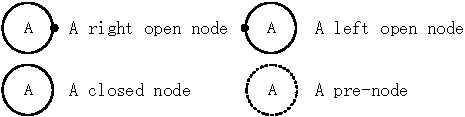
\includegraphics{partialtree/figures/fromWord-2.pdf}
\caption{Four types of element nodes}
\label{fig:nodetypes}
\end{figure}

%
%
\section{Characteristics of Partial Tree}
\label{sec:chars}

Now we discuss the Characteristics of partial trees. Since the left-open nodes,
right-open nodes and pre-nodes are most significant concept in partial trees, we
first focus on the properties of these open node.

\subsection{Properties of Open Nodes}

We introduce three properties of open nodes. The first property is about the
parent-child relationship of the open nodes.

\begin{property}
\label{property1}\itshape
If a node on a partial tree is left/right open, then its parent is also
left/right open.
\end{property}

The second property is about the sibling relationship of the open nodes.

\begin{property}
\label{property2}\itshape
If a node is left open, it is the first node among its
siblings in the partial tree. If a node is right open, it is the last
node among its siblings in the partial tree.
\end{property}

There is another important property of pre-nodes.

\begin{property}
\label{property3}\itshape
If there exist multiple pre-nodes, then only one of
them has left-open/closed/right-open nodes as its child.
\end{property}


\subsection{Standard Structure}

According the properties of partial tree, the standard structure of partial tree
can be described as in Fig.~\ref{fig:model}.

\begin{figure}[t]
\centering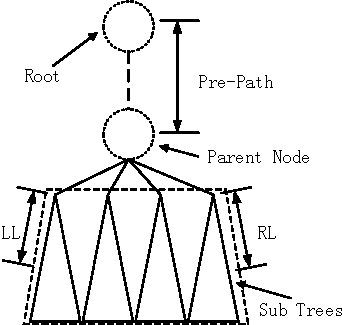
\includegraphics{partialtree/figures/fromWord-4.pdf}
\caption{The standard structure of partial tree.}
\label{fig:model}
\end{figure}

A partial tree consists vertically of two parts. The bottom part is a forest
of subtrees and the top part is a list of pre-open nodes denoting the path from
the root to the bottom part. We call the list of pre-open nodes emph{pre-path}.
Pre-path plays an important role in applying queries from the root. From
property~\ref{property3}, one or more subtrees connect to a pre-node at the
bottom of the pre-path. Note that for each subtree, there is only one root,
which is a left-open/closed/right-open node, but there could be one or more
subtrees.

From properties \ref{property1} and \ref{property2}, we know that left-open
nodes are located on the upper-left part of a partial tree and the right-open
nodes are located on the upper-right part. More precisely, the left-open nodes
form a list from a root node of a subtree, and we call the list the \emph{left
list} (LL). Likewise, we call the list of right-open nodes the \emph{right list}
(RL).

%
%
\def\INDEXSET#1{\mathit{#1}_{[P]}}
\def\baselinestretch{1.5}

\section{Construction of Partial Trees}
\label{sec:construction}

Since the structure of partial tree is quite different from ordinary XML trees,
especially the pre-path, ordinary XML parsing algorithms, in turn, do not work
for the construction of partial tree. The difference mainly lies in two aspects.
First, an XML document can generate only a single XML tree. While in case of
partial tree, the number of XML trees could be many, which is determined by the
number of chunks. However, we cannot simply construct an partial tree from a
chunk. This is caused by the second reason that the pre-path of a partial tree
is missing in the corresponding chunk.

For constructing the pre-path, it is important that a partial tree that
corresponds to a chunk is the minimum subgraph. It should satisfy the following
three conditions:

(1) the subgraph is connected (This means the subgraph is a tree.);

(2) each node in the chunk is in the subgraph, and

(3) the root of the original XML tree is in the subgraph.

For an intuitive grasp, we use the following XML document as the running
example.

\begin{quote}\tt\small
<A><B><C><E></E></C><D></D></B><E></E><B><B><D><E>\\
</E></D><C></C></B><C><E></E></C><D><E></E></D></B>\\
<E><D></D></E><B><D></D><C></C></B><B></B></A>\\
\end{quote}

From the document, we can construct an XML tree as shown in Fig.~\ref{fig:tree}.
We number all the nodes of the tree in a prefix order for identification.



To construct partial trees from the document, we first split it into five chunks
as listed below.

 chunk$_0$: \texttt{ <A><B><C><E></E></C><D></D></B>}

 chunk$_1$: \texttt{ <E></E><B><B><D><E></E></D>}

 chunk$_2$: \texttt{ <C></C></B><C><E></E></C><D>}

 chunk$_3$: \texttt{ <E></E></D></B><E><D></D></E>}

 chunk$_4$: \texttt{ <B><D></D><C></C></B><B></B></A> }


\begin{figure*}[t]
	\centering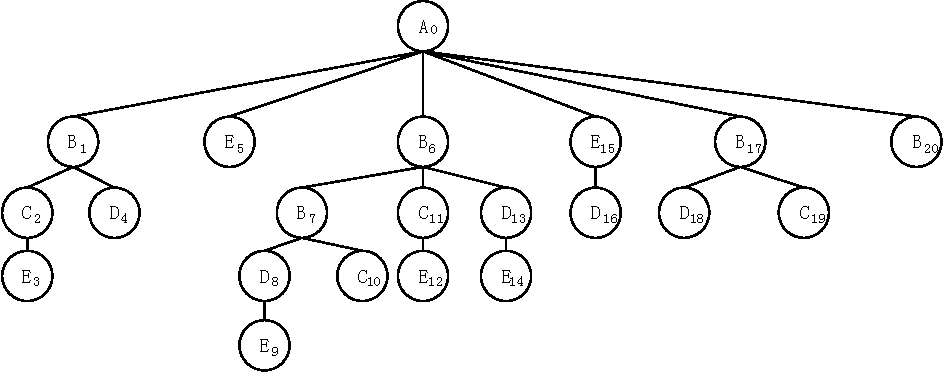
\includegraphics[scale=.9]{partialtree/figures/fromWord-5.pdf}
	\caption{an XML tree from the given XML string}
	\label{fig:tree}
	
	\centering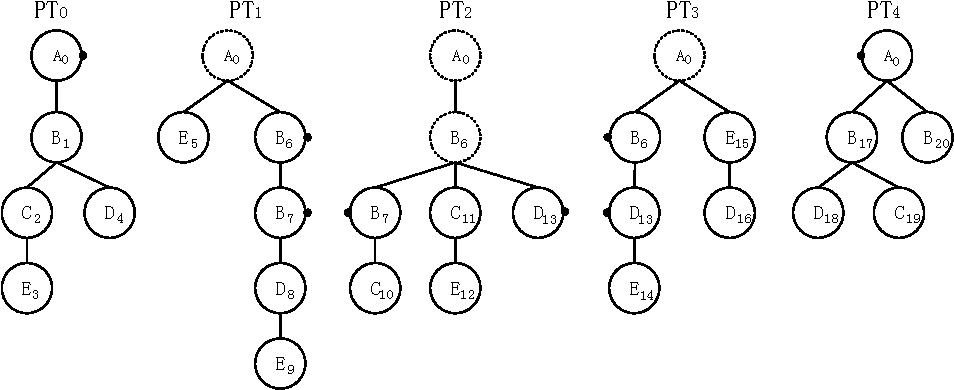
\includegraphics[scale=.9]{partialtree/figures/fromWord-7.pdf}
	\caption{Partial trees from the given XML string.}
	\label{fig:partialtree2}
\end{figure*}

We can construct a parital tree from each chunk, i.e. chunk$_i$ makes a partial
tree PT$_i$, as shown in Figure~\ref{fig:partialtree2}.

In the following section, we introduce our partial tree construction algorithm
with the example. Our algorithm is a three-phase algorithm. In the first phase,
we construct mutiple sets of subtrees that have some open nodes from parsing
chunks of the input XML document. Second, we compute pre-path for each list of
subtrees with all the open nodes. Last, we add pre-paths to the corresponding
list of subtrees to complete the partial tree construction. We will give deailed
introduction to the three-phase construction algorithm of partial tree.
Furthermore, to server the query algorithm, we also introduce the statistics
information of open nodes, called ranges of open nodes. With such information,
we can easily access open nodes of the same node and synchronize the query
results among partial trees.

\subsection{Construction of Subtrees From Parsing XML Chunks}

As introduced previously, a partial tree is constructed from parsing an input
XML chunk, which is a substring generated from splitting the XML document. We
design an algorithm that parses the input XML string into a similar tree by
using an iterative function with a stack, which is similar to ordinary XML
parsing algorithms.

First, after splitting an XML document, we deal with nodes with missing tags.
During parsing, we push start tags onto the stack. When we meet an end tag, we
pop a last start tag to merge a closed node. However, as a result of splitting,
some nodes miss their matching tags. In this case, we mark it left-open or
right-open based on which tag (either start tag or end tag) is missing. Then, we
add them onto the subtrees in the same way as we add closed nodes.

We also need to handle the case when the split position falls inside a tag and
thus splits the tag into two halves. In this case, we simply merge the split
tags. Because there are at most two split tags on a partial tree, the time taken
for merging them is negligible.

One or more subtrees can be constructed from a single chunk. For example, we
can construct nine subtrees from parsing the five chunks above as shown in
Fig.~\ref{fig:partialtree-notfinished}. Chunk$_0$ and chunk$_4$ have only one
subtree while chunk$_2$ has three subtrees. After the parsing phase, these
subtrees are used for pre-path computation.

\begin{figure*}[t]
	\centering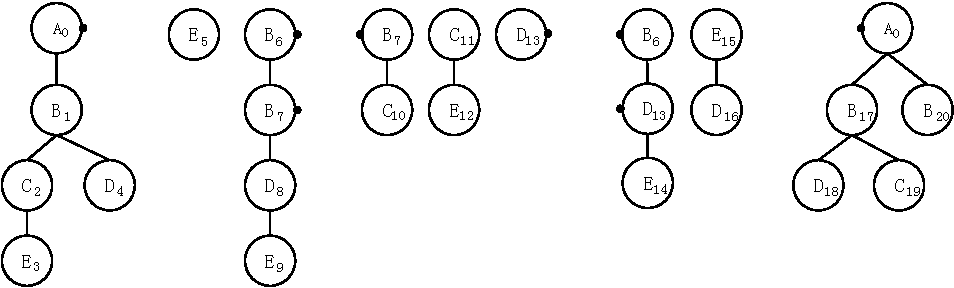
\includegraphics[]{partialtree/figures/fromWord-6.pdf}
	\caption{Subtrees from parsing chunks}
	\label{fig:partialtree-notfinished}
\end{figure*}


\subsection{Pre-path Computation}

The key idea of computing the pre-path for each partial tree is to make use
of open nodes. This is because the missing parent and ancestor nodes are caused
by splitting those nodes. Therefore, the information needed for creating the
pre-paths lies in them.

Algorithm 0 outlines the pseudo codes for computing pre-path. Since one chunk
may generate more than one subtrees, the input is a list of subtree lists. The
length of the list is equal to the number of partial trees, i.e. one chunk makes
one list of subtree, thus representing the length as $P$.

Algorithm 0 has three phases. In the first phase, it selects all the left-open
nodes into $LLS$ and all the right-open nodes into $RLS$ (line 2-4). $LLS_{[P]}$
collects the left-open nodes of the $p$th partial tree, likewise we have
$RLS_{[P]}$. Note that the nodes in $LLS_{[P]}$ or $RLS_{[P]}$ are arranged in
order from the root to leaves. For example, in Table~\ref{table:opennodes}, we
select all the open nodes and add them to corresponding lists.

{
	\setstretch{1.5}
\begin{figure}[!t]
 	\centering
 	\label{fig:ppalgorithm}
 	\begin{tabular}{l}
 		\hline
 		\hline
 		\makebox[.95\linewidth][l]{\textbf{Algorithm 0} \textsc{GetPrepath}($\mathit{STS}$)} \\
 		\hline
 		\textbf{Input}: $\mathit{STS}$: a list of subtree lists \\
 		\textbf{Output}: an list of partial trees\\
 		\makebox[1em][r]{1:}\hspace{1 mm} /* open nodes in LLS or RLS are arranged in top-bottom order */\\
 		\makebox[1em][r]{2:}\hspace{1 mm} \textbf{for all} $p \in [0, P)$ \textbf{do} \\
 		\makebox[1em][r]{3:}\hspace{4 mm} $\INDEXSETL{LLS} \leftarrow \mathit{SelectLeftOpenNodes}(\INDEXSETL{STS})$\\
 		\makebox[1em][r]{4:}\hspace{4 mm} $\INDEXSETL{RLS} \leftarrow \mathit{SelectRightOpenNodes}(\INDEXSETL{STS})$\\

 		\makebox[1em][r]{5:}\hspace{1 mm} /* Prepath-computation and collecting matching nodes */\\
 		\makebox[1em][r]{6:}\hspace{1 mm} $AuxList \leftarrow []$ \\
 		\makebox[1em][r]{7:}\hspace{1 mm} \textbf{for} $ p \in [0, P-1) $ \textbf{do}\\
 		\makebox[1em][r]{8:}\hspace{4 mm} $AuxList.\mathit{AppendToHead}(\INDEXSETL{RLS})$\\
 		\makebox[1em][r]{9:}\hspace{4 mm} $AuxList.\mathit{RemoveLast}(LLS_{[p+1]}.\mathit{Size}()) $\\
 		\makebox[1em][r]{10:}\hspace{4 mm} $ PPS_{[p+1]}\leftarrow AuxList$ \\

 		\makebox[1em][r]{11:}\hspace{1 mm}  /* Add pre-nodes to subtrees */ \\
 		\makebox[1em][r]{12:}\hspace{1 mm} $PTS \leftarrow []$ \\
 		\makebox[1em][r]{13:}\hspace{1 mm} \textbf{for} $ p \in [0, P) $ \textbf{do}\\
 		\makebox[1em][r]{14:}\hspace{4 mm} \textbf{for} $ i \in [0, PPS_{[p]}.Size() - 1)$ \textbf{do} \\
 		\makebox[1em][r]{15:}\hspace{8 mm}   $PPS_{[p][i]}.children.$Add$(PPS_{[p][i+1]})$ \\
  		\makebox[1em][r]{16:}\hspace{4 mm} $PPS_{[p]}.last.children.$Add$(\INDEXSETL{STS})$ \\
 		\makebox[1em][r]{17:}\hspace{4 mm}   $\INDEXSETL{PTS} \leftarrow PPS_{[p][0]}$ \\
 		\makebox[1em][r]{18:}\hspace{1 mm} \textbf{return} \emph{PTS} \\
 		\hline
 	\end{tabular}
 \end{figure}
}

In the second phase, we perform the pre-path computation. Once we split an XML
document from a position inside the document, the two partial trees created from
the splitting have the same number of open nodes on the splitting side. Given
two consecutive partial trees, the number of the right-open nodes of the left
partial tree is the same as the number of the left-open nodes of the right
partial tree. This is a very important feature and we exploit it for computing
the pre-paths of partial trees.

In the algorithm, we first add the $p$th $RLS$ to the head of an auxiliary list
$AuxList$ (line 8), and then we remove the same number of nodes as the number of
$(p-1)$th $LLS$ (line 9). Last, we keep the nodes in the $AuxList$ to the
$(p+1)$th $PPS$, which holds the pre-nodes for each partial tree.
Table~\ref{table:tempresult} shows the results of pre-path computation for the
given example.

{
\setstretch{1.5}
\begin{table}[t]
	\caption{Open node lists}
	\label{table:opennodes}
	\centering
	\begin{tabular}{c|cc}
		\hline
		& Left-open nodes	& Right-open nodes \\
		\hline
		pt$_0$	& []			& [A$_0$] \\
		pt$_1$	& []			& [B$_6$, B$_7$] \\
		pt$_2$	& [B$_7$]			& [D$_1$$_3$] \\
		pt$_3$	& [B$_6$, D$_1$$_3$]		& [] \\
		pt$_4$	& [A$_0$]			& [] \\
		\hline
	\end{tabular}

	\caption{Results of pre-path computation in AUX}
	\label{table:tempresult}
	\centering
	\begin{tabular}{c|ccc}
		\hline
		& Left-open nodes	& Right-open nodes & $AUX$\\
		\hline
		pt$_0$	& []			& [A$_0$]  & []\\
		pt$_1$	& []			& [B$_6$, B$_7$] & [A$_0$] \\
		pt$_2$	& [B$_7$]			& [D13] &[A$_0$,B$_6$]\\
		pt$_3$	& [B$_7$, D$_1$$_3$]		& []  & [A$_0$]\\
		pt$_4$	& [A$_0$]			& [] &[]\\
		\hline
	\end{tabular}
\end{table}
}

In last phase, we add the resultant pre-nodes to the corresponding partial trees
and copy the nodes from $PPS_{[p]}$ to $PTS_{[p]}$ as the results for output.
Because the pre-nodes in the pre-path are also open nodes, we list all open
nodes for each partial trees in Table~\ref{table:allopennodes}. Then, the
pre-path computation is complete. For the given example, we obtain the partial
trees as shown in Fig.~\ref{fig:partialtree2}.


\subsection{Creation of Ranges of Open Nodes}
\label{sec:ranges}

Once an XML node is split, it generates two or more open nodes of the same node
in consecutive partial trees. For example, as we can see in
Fig.~\ref{fig:partialtree2}, \Nr{B}{6} on pt$_1$, \Np{B}{6} on pt$_2$, and
\Nl{B}{6}  on pt$_3$ are created from the same node \Nc{B}{6}. For locating the
open nodes of the same node,  which are distrubted in different partial trees,
we use two integers \textit{start} and \textit{end} for an open node. With these
two integers, we can know the partial trees that have matching nodes of the same
open node. Note that after adding nodes to a partial tree, the open nodes from
the same node also have the same depth. Therefore, we can locate all the
matching nodes to set \textit{start} and \textit{end} for each open node. After
computation, we obtain the ranges of nodes as shown in
Table~\ref{table:rangesresult}.

{
	\setstretch{1.5}
\begin{table}[t]
		\caption{All open nodes}
	\label{table:allopennodes}
	\centering
	\begin{tabular}{c|cc}
		\hline
		& Left-open nodes	& Right-open nodes \\
		\hline
		pt$_0$	& []						& [A$_0$] \\
		pt$_1$	& [A$_0$]					& [A$_0$, B$_6$, B$_7$] \\
		pt$_2$	& [A$_0$, B$_6$, B$_7$]		& [A$_0$, B$_6$, D$_1$$_3$] \\
		pt$_3$	& [A$_0$, B$_6$, D$_1$$_3$]	& [A$_0$] \\
		pt$_4$	& [A$_0$]					& [] \\
		\hline
	\end{tabular}

	\caption{Open node lists with ranges}
	\label{table:rangesresult}
	\centering
	\begin{tabular}{c|cc}
		\hline
		& Left open nodes	& Right open nodes \\
		\hline
		pt$_0$	& []	& [A$_0$(0,4)] \\
		pt$_1$	& [A$_0$(0,4)]	& [A$_0$(0,4), B$_6$(1,3), B$_7$(1,2)] \\
		pt$_2$	& [A$_0$(0,4), B$_6$(1,3), B$_7$(1,2)]	& [A$_0$(0,4), B$_6$(1,3), D$_1$$_3$(2,3)] \\
		pt$_3$	& [A$_0$(0,4), B$_6$(1,3), D$_1$$_3$(2,3)]	& [A$_0$(0,4)] \\
		pt$_4$	& [A$_0$(0,4)]	& [] \\
		\hline
	\end{tabular}
\end{table}
}

By using these ranges, we can esaily establish the partial trees for the
matching nodes of the same node. For example, the range of A$_0$ is (0, 4), that
means we can locate the same nodes of \Nc{A}{0} from pt$_0$ to pt$_4$. As we can
see, there are \Nr{A}{0}, \Np{A}{0}, \Np{A}{0}, \Np{A}{0}, and \Nr{A}{0} on
pt$_0$ to pt$_4$, respectively.

%
%\section{Eavalute XPath Queries on Partial Trees}
\label{sec:queryalgo}

When performing an XPath query on an XML document, the evaluation is done on a
single tree. By exploiting partial tree, the evaluation of an XPath query on a
single tree is then applied to multiple partial trees. A significant advantagte
of using partial tree is that it makes the parallelization of evaluation of
XPath queries possible by simply evaluting the same query on partail trees
separately. However, it also brings challenges in designing query algorhtms on
partial trees. Generally speaking, there are three main difficulties as follows.

First, since partial trees are craeted from chunks of an XML document, a node
may be seperated and thus lie in different partial trees. This leads to a
possible situation that multiple open nodes may stem from the same node and
distributed in different partial trees as discussed in Section~\ref{sec:ranges}.
Since these open nodes are from the same node, in case when one of such open
nodes is selected in a partial tree (e.g., \Nr{B}{6} on \PT1), the other
corresponding nodes (\Np{B}{6} on \PT2 and \Nl{B}{6} on \PT3) should also be
selected for consistency. This is simply because they are all \Nc{B}{6} in the
original XML document.

Second, although partial trees have all the parent-child edges of their nodes,
the sibling-relation that is split among partial trees may be missing. For
example,  \Nc{B}{1} has five following-sibling nodes in the original XML tree,
but in \PT1, there is no following-sibling nodes of \Nc{B}{1} because of
splitting. When we perform queries with \texttt{following-sibling} or
\texttt{preceding-sibling}, the results may be in another (possibly far) partial
tree. We  design an algorithm to let the partial trees know about such cases.

Third, when we perform queries with a predicate, we usually execute the
sub-query in the predicate from a set of matching nodes.  However, on a set of
partial trees, the starting nodes and the matching nodes of the sub-query may be
on different partial trees (we will show this in the follwoing part of this
section). We also need an algorithm to propagate the information over partial
trees for queries with predicates.

In this section, we develop algorithms for evaluating XPath queries on a set of
partial trees. We first show the outline of the algorithms and then describe the
details of how the query algorithms work for evaluating XPath queries. We use
the following three XPath expressions as our running examples.

Q1: \texttt{ /child::A/descendant::B/descendant::C/parent::B}

Q2: \texttt{ /descendant::B/following-sibling::B}

Q3:  \texttt{ /descendant::B[following-sibling::B/child::C]/child::C}

After the introduction of the algorithms, we also discuss the complexity of our
algorithms at the end of this section.


\subsection{Definitions}

For introducing the query algorithms, we first give a few definitions to partial
tree nodes. Each node has a \textit{type} denoting its node type, including
closed, left-open, right-open and pre-node, and \textit{depth} denoting the
number of edges from the node to the root. A node has four pointers pointing to
the related nodes: the \textit{parent} pointer that points to its parent and the
\textit{children} pointer to its children. For accessing siblings, it has the
\textit{presib} pointer and the \textit{folsib} pointer that points to its
preceding-sibling node and following-sibling node, respectively. For
distinguishing nodes, we give each node a unique id called \textit{uid}.

Besides the partial tree node, there is also a requirement that we need to know
from which partial tree a node comes in distributed memory environments;
therefore, we number each partial tree with a unique id denoted as
\textit{partial tree id} or simply \textit{ptid} for distinguishing partial
trees. We number \textit{ptid} from 0 to \textit{P - 1} (where P is the total
number of partial trees) in document order.

For locating any node on a partial tree, we define data type \textit{Link} that
holds a ptid and a uid. By using \textsc{FindNode}(\textit{pt}, \textit{uid}),
we can locate any node with a unique integer \textit{uid} on partial tree
\textit{pt}. We assume that we can access any node in constant time.

When processing an XPath query, we evaluate it step by step in order. For
storing the results of a step, we define a resultant list of nodes for each
partial tree i.e. the are P reslultant lists given P partial trees. The
evaluation of a step is applies to each node in the resultant list. To start
with, we add a virtual node VN$i$ into a resultant list for each parital tree,
which has the root of PT$i$ as its single child. For example, VN$_0$ has only a
single child \Nr{A}{0} of \PT0 and is put into the resultant list before the
evaluation on \PT0 starts. The evaluation of a step generats a new resultant
list of nodes. After the evaluation, we replace the current resultant list with
the new list as the results and will be used as the input for the next step.


\subsection{Queries without Predicate}

Algorithm~1 outlines the big picture of our XPath query algorithms. The input
includes an XPath query to be evaluated and a set of partial trees generated
from an XML document. The output is a set of resultant nodes that matchs the
XPath query, each of which is associated with a corresponding partial tree.

The evaluation of the XPath query starts from the root of the original XML tree.
In case of paritial tree, the root node of the original tree corresponds to the
root node of every partial tree, and they are put into the resultant lists for
holding intermediate results (lines 1--2). Hereafter, the loops by $p$ over $[0,
P)$ are assumed to be executed in parallel.

As we know, an XPath query consists of one or more location steps, and in our
algorithm they are processed one by one in order. For each step, Algorithm~1
calls the corresponding sub-algorithm based on the axis of the step and updates
the intermediate results (line 4) in the resultant lists for each turn. Lines
6--9 will be executed in case the input XPath query has a predicates. We will
explain this part later in Section~\ref{sec:predicate}.

{
	\setstretch{1.5}
\begin{figure}[t]
  \label{fig:algQuery2}
	\centering
	\begin{tabular}{l}
		\hline
		\hline
		\makebox[.95\linewidth][l]{\textbf{Algorithm 1} \textsc{Query}($\mathit{steps}$, $\INDEXSET{pt}$)} \\
		\hline
		\textbf{Input}:           $\mathit{steps}$: an XPath expression \\
                \phantom{\textbf{Input}:} $\INDEXSET{pt}$: an indexed set of partial trees \\
		\textbf{Output}: an indexed set of results of query \\
		\makebox[1em][r]{1:}\hspace{1 mm} \textbf{for} $p \in [0, P)$ \textbf{do} \\
		\makebox[1em][r]{2:}\hspace{4 mm}    $\mathit{ResultList}_p \leftarrow \{~ \mathit{pt}_p.\mathit{root} ~\}$ \\
		\makebox[1em][r]{3:}\hspace{1 mm} \textbf{for all} $\emph{step} \in \emph{steps}$ \textbf{do} \\
		\makebox[1em][r]{4:}\hspace{4 mm}    $\INDEXSET{ResultList}$ \\
                \makebox[1em][r]{  }\hspace{6 mm}        ${}\leftarrow \hbox{\textsc{Query}}\langle\mathit{step}.\mathit{axis}\rangle(\INDEXSET{pt}, \INDEXSET{ResultList}, \mathit{step}.\mathit{test})$ \\
		\makebox[1em][r]{5:}\hspace{4 mm}    \textbf{if} $step.predicate \neq \hbox{\textsc{null}}$ \textbf{then} \\
		\makebox[1em][r]{6:}\hspace{7 mm}       $\INDEXSET{PResultList} \leftarrow \hbox{\textsc{PreparePredicate}}(\INDEXSET{ResultList})$ \\
		\makebox[1em][r]{7:}\hspace{7 mm}       \textbf{for all} $\emph{pstep} \in \emph{step.predicate}$ \textbf{do} \\
		\makebox[1em][r]{8:}\hspace{10 mm}         $\INDEXSET{PResultList}$ \\
                \makebox[1em][r]{  }\hspace{12 mm}             ${} \leftarrow  \hbox{\textsc{PQuery}}\langle\mathit{step}.\mathit{axis}\rangle(\INDEXSET{pt}, \INDEXSET{PResultList}, \mathit{pstep})$ \\
		\makebox[1em][r]{9:}\hspace{7 mm}       $\INDEXSET{ResultList} \leftarrow \hbox{\textsc{ProcessPredicate}}(\INDEXSET{PResultList})$ \\
		\makebox[1em][r]{10:}\hspace{1 mm} \textbf{return} $\INDEXSET{ResultList}$ \\
		\hline
	\end{tabular}
  \caption{Overall algorithm of XPath query for partial trees}
\end{figure}
}


\subsubsection{Downwards Axes}

Algorithm 2 shows the procedure for evaluting a step with a child axis. The
input $\INDEXSET{InputList}$ has the nodes selected up from the last step on
each partial tree. The algorithm simply lists up all the children of input nodes
and compares their tags with the node test (lines 3--4).

Algorithm 3 shows the procedure for evaluting a step with a descendant axis.
Starting from every node in the input, it traverses partial trees by depth-first
search along with a stack. To avoid redundant traversals on the same node, we
add the $\mathit{isChecked}$ flag for each node (lines 8--9) so that we can
evaluate  each node only once. Note that we can reduce the worst-case complexity
by using this flag from square to linear with respect to the number of nodes.

{
	\setstretch{1.5}
\begin{figure}[!t]
	\centering
	\begin{tabular}{l}
		\hline
		\hline
		\makebox[.95\linewidth][l]{\textbf{Algorithm 2} \textsc{Query}$\langle$\texttt{child}$\rangle$($\INDEXSET{pt}$, $\INDEXSET{InputList}$, $\mathit{test}$)} \\
		\hline
		\textbf{Input}:           $\INDEXSET{pt}$: an indexed set of partial trees \\
                \phantom{\textbf{Input}:} $\INDEXSET{InputList}$: an indexed set of input nodes \\
                \phantom{\textbf{Input}:} $\mathit{test}$: a string of nametest \\
		\textbf{Output}: an indexed set of results \\
		\makebox[1em][r]{1:}\hspace{1 mm} \textbf{for} $p \in [0, P)$ \textbf{do} \\
		\makebox[1em][r]{2:}\hspace{4 mm}    $\mathit{OutputList}_p \leftarrow [] $ \\
		\makebox[1em][r]{3:}\hspace{4 mm}    \textbf{for all} $n \in InputList_p$ \textbf{do} \\
		\makebox[1em][r]{4:}\hspace{7 mm}       $\mathit{OutputList}_p $ \\
                \makebox[1em][r]{  }\hspace{9 mm}          ${}\leftarrow \mathit{OutputList}_p \cup [nc ~|~ nc \in n.\mathit{children}, nc.\mathit{tag} = \mathit{test}] $ \\
		\makebox[1em][r]{5:}\hspace{1 mm} \textbf{return} $\INDEXSET{OutputList}$ \\
		\hline
        \\
		\hline
		\hline
		\makebox[.95\linewidth][l]{\textbf{Algorithm 3} \textsc{Query}$\langle$\texttt{descendant}$\rangle$($\INDEXSET{pt}$, $\INDEXSET{InputList}$, $\mathit{test}$)} \\
		\hline
		\textbf{Input}:           $\INDEXSET{pt}$: an indexed set of partial trees \\
                \phantom{\textbf{Input}:} $\INDEXSET{InputList}$: an indexed set of input nodes \\
                \phantom{\textbf{Input}:} $\mathit{test}$: a string of nametest \\
		\textbf{Output}: an indexed set of results \\
		\makebox[1em][r]{1:}\hspace{1 mm} \textbf{for} $p \in [0, P)$ \textbf{do} \\
		\makebox[1em][r]{2:}\hspace{4 mm}    $\mathrm{SetIsChecked}(\mathit{pt}_p, \mathit{false})$ \\
		\makebox[1em][r]{3:}\hspace{4 mm}    $\mathit{OutputList} \leftarrow [] $ \\
		\makebox[1em][r]{4:}\hspace{4 mm}    \textbf{for all} $n \in InputList_p$ \textbf{do} \\
		\makebox[1em][r]{5:}\hspace{7 mm}       $\mathit{Stack} \leftarrow \{ \emph{n} \}$ \\
		\makebox[1em][r]{6:}\hspace{7 mm}       \textbf{while not }$\mathit{Stack}.\mathit{Empty()}$ \textbf{do}  \\
		\makebox[1em][r]{7:}\hspace{10mm}         $nt \leftarrow \mathit{Stack}.\mathit{Pop}()$  \\
		\makebox[1em][r]{8:}\hspace{10mm}         \textbf{if} $nt.\mathit{isChecked}$ \textbf{then} \textbf{continue} \\
		\makebox[1em][r]{9:}\hspace{10mm}         $nt.\mathit{isChecked} \leftarrow \hbox{\textsc{true}}$ \\
		\makebox[1em][r]{10:}\hspace{10mm}         $\mathit{OutputList}_p $ \\
                \makebox[1em][r]{   }\hspace{12mm}             ${}\leftarrow \mathit{OutputList}_p \cup [nc ~|~ nc \in nt.children, nc.\mathit{tag} = \mathit{test}] $ \\
		\makebox[1em][r]{11:}\hspace{10mm}         $\mathit{Stack}.\mathit{PushAll}(nt.\mathit{children})$ \\
		\makebox[1em][r]{12:}\hspace{1 mm} \textbf{return} $\INDEXSET{OutputList}$ \\
		\hline
	\end{tabular}
    \caption{Query algorithm for downwards axes}
	\label{fig:algQueryChild2}
\end{figure}
}

Now let us look at our running example Q1. The process of downward steps of Q1
is listed in Table~\ref{tab:Q1first}. For the first step \texttt{child::A},
since  VN$_i$ has only one child that is the root of the $i$th partial tree, we
obtain it as the results for each partial tree as shown in the second row of the
table. Then we perform the next step \texttt{descendant::B} independently for
each partial tree from the results of the first step. We evalute the step
\texttt{descendant::B} on each of the nodes in the resultant list of the
previous step. For example, for \Nr{A}{1} on \PT1, there is only a node
\Nc{B}{1} that matches the query and is then selected and put into a new list.
As introduced, when the evaluation is done, the new list replaces the current
resultant list to be the resultant list up to the current step. The results of
this step for each partial tree are listed in the fourth row of
Table~\ref{tab:Q1first}.  For the third step \texttt{descendant::C}, the
algorithm works in a similar way. The results up to \texttt{descendant::C} are
lised in the last row of Table~\ref{tab:Q1first}. It is worth noting that the
$\mathit{isChecked}$ flag now works. For example, on \PT1, starting from
\Nr{B}{6}, we traverse \Nr{B}{7}, \Nc{D}{8}, \Nc{E}{9}, and then starting from
\Nr{B}{7}, we can stop the traversal immediately.

{
\setstretch{1.5}
\begin{table}[t]
\caption{Evaluating downward steps of Q1}
\label{tab:Q1first}
\begin{center}
\begin{tabular}{c|ccccc}
\hline
\hline
Process &
\PT0 &
\PT1 &
\PT2 &
\PT3 &
\PT4 \\
\hline
Input&
[VN$_0$] &
[VN$_1$] &
[VN$_2$] &
[VN$_3$] &
[VN$_4$] \\
\hline
\texttt{child::A} &
$ [\Nr{A}{0}] $ &
$ [\Np{A}{0}] $ &
$ [\Np{A}{0}] $ &
$ [\Np{A}{0}] $ &
$ [\Nl{A}{0}] $ \\
\hline
\texttt{descendant::B} &
$ [\Nc{B}{1}] $ &
$ [\Nr{B}{6}, \Nr{B}{7}] $ &
$ [\Np{B}{6}, \Nl{B}{7}] $ &
$ [\Nl{B}{6}] $ &
$ [\Nc{B}{17}, \Nc{B}{20}] $ \\
\hline
\texttt{descendant::C} &
$ [\Nc{C}{2}] $ &
$ [\,] $ &
$ [\Nc{C}{10}, \Nc{C}{11}] $ &
$ [\,] $ &
$ [\Nc{C}{19}] $ \\
\hline
\end{tabular}
\label{tab:Q1}
\end{center}
\end{table}
}

\subsubsection{Upwards Axes}

In querying of a step with downward axes, the algorithms have nothing different
to partial trees compared to ordinary XML trees. This is due to Property 1 in
Section~\ref{sec:chars}. Let an open node $x$ be selected after a downwards
query. Then, it should have started from an open node (this is an ancestor of
$x$) and the corresponding nodes should have all been selected, which means all
the nodes corresponding to $x$ should be selected after the query.

However, this discussion does not hold for the queries with upwards axes. In
such case when an open node is selected after an upwards query, it may come
from a closed node and we have no guarantee that all the corresponding open
nodes are selected. Therefore, we add a postprocessing for sharing the selected
nodes when we process the upwards axes.

Algorithm 4 shows the procedure for evaluating a step with a parent axis.
It has almost the same flow as that of the child axis (lines 1--5),
except for the last call of the \textsc{ShareNodes} function.

The \textsc{ShareNodes} function is used for keeping the consistency of open
nodes. It consists of two parts\footnote{In our implementation of this
\textsc{ShareNodes} function, there are two phases of communication: all the
partial trees send their open nodes to a process and then the necessary data for
a partial tree are sent back.}.

First, it collects all the selected open nodes from all partial trees (lines
4--6). Then, based on the range information of node $n$ ($n.\mathit{start}$ and
$n.\mathit{end}$), we add all the corresponding selected nodes to all the
partial trees. After the call of \textsc{ShareNodes} function, all the open
nodes that are from the same node are selected in corresponding partial trees.

Now, let us continue the running example Q1 for its last step as shown in
Table~\ref{tab:Q1last}. For the \texttt{parent::B} after the
\texttt{descendant::C}, we first directly select the parent nodes of the
intermediate results from the results of the previous step independently. For
the running example, we can notice that \Nc{B}{1} is selected for it is  the
parent of \Nc{C}{2} on \PT0, while for \Nl{B}{7} and \Np{B}{6}, they are the
parents of \Nc{C}{10} and \Nc{C}{11} respectively.  The results are listed in
the second row of Table\ref{tab:Q1last}.

Here, unfortunately the node \Nl{B}{7} is selected on \PT2, but its
corresponding node on \PT1, i.e. \Nr{B}{7}, has not been selected yet.  We then
call the \textsc{ShareNodes} function. By collecting all the open nodes from all
the partial trees, we have the list $[\Nl{B}{7}, \Np{B}{6}]$. Since they have
ranges $(1, 2)$ and $(1, 3)$, respectively, \PT1 receives two nodes \Nr{B}{7}
and \Nr{B}{6}, \PT2 receives two nodes \Nl{B}{7} and \Np{B}{6}, and \PT3
receives one node \Nl{B}{6}. By taking the union with the previous intermediate
results, we obtain the final results as shown in the last row of
Table\ref{tab:Q1last}.

Now, after evaluating the last step of Q1, the evaluation of the whole query Q1
is complete. The resultant lists in the last row of the table from evaluating
the last step is then the final results of Q1.

{
	\setstretch{1.5}
\begin{table}[t]
	\caption{Evaluating the last step of Q1}
	\label{tab:Q1last}
	\begin{center}
		\medskip
		\begin{tabular}{c|ccccc}
			\hline
			\hline
			Process &
			\PT0 &
			\PT1 &
			\PT2 &
			\PT3 &
			\PT4 \\
			\hline
			Input &
			$ [\Nc{C}{2}] $ &
			$ [\,] $ &
			$ [\Nc{C}{10}, \Nc{C}{11}] $ &
			$ [\,] $ &
			$ [\Nc{C}{19}] $ \\
			\hline
			\texttt{parent::B} &
			$ [\Nc{B}{1}] $ &
			$ [\,] $ &
			$ [\Nl{B}{7}, \Np{B}{6}] $ &
			$ [\,] $ &
			$ [\Nc{B}{17}] $ \\
			\hline
			\textsc{ShareNode} &
			$ [\Nc{B}{1}] $ &
			$ [\Nr{B}{6}, \Nr{B}{7}] $ &
			$ [\Nl{B}{7}, \Np{B}{6}] $ &
			$ [\Nl{B}{6}] $ &
			$ [\Nc{B}{17}] $ \\
			\hline
		\end{tabular}
		\medskip
	\end{center}
\end{table}

\begin{figure}[t]
	\centering
	\begin{tabular}{l}
		\hline
		\hline
		\makebox[.95\linewidth][l]{\textbf{Algorithm 4} \textsc{Query}$\langle$\texttt{parent}$\rangle$($\INDEXSET{pt}$, $\INDEXSET{InputList}$, $\mathit{test}$)} \\
		\hline
		\textbf{Input}:           $\INDEXSET{pt}$: an indexed set of partial trees \\
        \phantom{\textbf{Input}:} $\INDEXSET{InputList}$: an indexed set of input nodes \\
        \phantom{\textbf{Input}:} $\mathit{test}$: a string of nametest \\
		\textbf{Output}: an indexed set of results \\
		\makebox[1em][r]{1:}\hspace{1 mm} \textbf{for} $p \in [0, P)$ \textbf{do} \\
		\makebox[1em][r]{2:}\hspace{4 mm}    $\mathit{OutputList}_p \leftarrow [\,]$ \\
		\makebox[1em][r]{3:}\hspace{4 mm}    \textbf{for all} $n \in \mathit{InputList}_p$ \textbf{do} \\
		\makebox[1em][r]{4:}\hspace{7 mm}       \textbf{if} $n.\mathit{parent} \neq \hbox{\textsc{null}}$ \textbf{ and } $n.\mathit{parent}.\mathit{tag} = \emph{test}$ \textbf{then} \\
		\makebox[1em][r]{5:}\hspace{10mm}          $\mathit{OutputList}_p.\mathit{Add}(n)$ \\
		\makebox[1em][r]{6:}\hspace{1 mm} \textbf{return} \textsc{ShareNodes}($\INDEXSET{pt}$, $\INDEXSET{OutputList}$) \\
		\hline
        \\
        \hline
		\hline
		\makebox[.95\linewidth][l]{\textbf{Algorithms 5} \textsc{ShareNodes}($\INDEXSET{pt}$, $\INDEXSET{NodeList})$} \\
		\hline
		\textbf{Input}:           $\INDEXSET{pt}$: an indexed set of partial trees \\
                \phantom{\textbf{Input}:} $\INDEXSET{NodeList}$: an indexed set of nodes \\
		\textbf{Output}: an indexed set of nodes after sharing\\
		\makebox[1em][r]{1:}\hspace{1 mm} /* Select all open nodes and append them to a node list */ \\
		\makebox[1em][r]{2:}\hspace{1 mm} $\mathit{ToBeShared} \leftarrow [\,]$ \\
		\makebox[1em][r]{3:}\hspace{1 mm} \textbf{for} $p \in [0, P)$ \textbf{do} \\
		\makebox[1em][r]{4:}\hspace{4 mm} $ \mathit{OpenNodes} \leftarrow [n ~|~ n \in \mathit{NodeList}_p, $\\
		\makebox[1em][r]{5:}\hspace{4 mm} \phantom{$ \mathit{OpenNodes} \leftarrow [n ~|~$}$n.\mathit{type} \in \{\textsc{LeftOpen}, \textsc{RightOpen}, \textsc{PreNode}\}]$\\
		\makebox[1em][r]{6:}\hspace{4 mm} $ \mathit{ToBeShared} \leftarrow \mathit{ToBeShared} \cup \mathit{OpenNodes}$ \\[5pt]
		\makebox[1em][r]{7:}\hspace{1 mm} /* Regroup nodes by partial tree id and add them to NodeList */ \\
		\makebox[1em][r]{8:}\hspace{1 mm} \textbf{for} $p \in [0, P)$ \textbf{do} \\
		\makebox[1em][r]{9:}\hspace{4 mm}    $\mathit{ToBeAdded}_p \leftarrow [n ~|~ n \in \mathit{ToBeShared}, n.\mathit{start} \le p \le n.\mathit{end}]$ \\
		\makebox[1em][r]{10:}\hspace{4 mm}    $\mathit{OutputList}_p \leftarrow \mathit{NodeList}_p \cup \mathit{ToBeAdded}_p$ \\
		\makebox[1em][r]{11:}\hspace{1 mm} \textbf{return} $\INDEXSET{OutputList}$ \\
		\hline
	\end{tabular}
        \caption{Query algorithms for upwards axes}
	\label{fig:algQueryParent2}
\end{figure}
}

\subsubsection{Intra-sibling Axes}

The \texttt{following-sibling} or \texttt{preceding-sibling} axes retrieve nodes
from a set of nodes that are siblings of an intermediate node.  In our partial
trees, a set of those sibling nodes might be divided into two or more partial
trees. Therefore, these intro-sibling axes require querying on other partial
trees in addition to the local querying.

Without loss of generality, we discuss the following-sibling axis only, since
preceding-sibling is only different in a opposite direction compared to
following-sibling axis. Algorithm 6 shows the procedure for evaluating a step
with a following-sibling axis, which consists of four phases: local query,
preparation, regrouping, and remote query.

In the local query, we utilize the $\mathit{folsib}$ pointer and the
$\mathit{isChecked}$ flag to realize linear-time querying (lines 6--10). Then,
in the preparation, we select the nodes that are passed to another partial tree
to perform the remote query.  The latter two conditions (lines 14, 15) are
rather easy: we will ask a remote query if the parent node can have more
segments on the right (i.e., right open). The former condition (line 13) is a
little tricky.  Even if the latter two conditions hold, we do not need a remote
query if the node itself is right open.  Notice that if a node is right open
then it should have a corresponding left-open node in another partial tree, and
that node will ask for a remote query.  The regrouping is almost the same as
that in \textsc{ShareNodes}, and the difference is the range we consider (we
only look at the right for the following-sibling). Finally, the remote query
finds the children from the intermediate nodes given by regrouping.

Now, let us look at our running example of Q2. After the evaluation of
\texttt{descendant::B}, we have the intermediate results in the third row of
Table~\ref{tab:query2}. In the first phase of \texttt{following-sibling::B}, we get
the results in the third row. Then, we collect the parent nodes that satisfies
the conditions (lines 13--15). Such nodes and their ranges are: \Nr{A}{0} with
range [1,4] (on \PT0), \Np{B}{6} with range [3,3] (on \PT2), and \Np{A}{0} with
range [4,4] (on \PT3). By regrouping the nodes based on the partial tree id, the
input nodes for the remote query are as in the fourth row of the table. Starting
from these intermediate results, we select their children and obtain the results
as shown in the last row of Table~\ref{tab:query2}. Note that these results are also
the final results for the query since the result of a local query is a subset of
this remote query.

{
	\setstretch{1.5}
\begin{table}[t]
	\caption{Evaluating the location steps of Q2}
	\label{tab:query2}
\centering
\small
\begin{tabular}{c|ccccc}
\hline
\hline
Process &
\PT0 &
\PT1 &
\PT2 &
\PT3 &
\PT4 \\
\hline
Input&
[VN$_0$] &
[VN$_1$] &
[VN$_2$] &
[VN$_3$] &
[VN$_4$] \\
\hline
\texttt{descendant::B} &
$ [\Nc{B}{1}] $ &
$ [\Nr{B}{6}, \Nr{B}{7}] $ &
$ [\Np{B}{6}, \Nl{B}{7}] $ &
$ [\Nl{B}{6}] $ &
$ [\Nc{B}{17}, \Nc{B}{20}] $ \\
\hline
\texttt{following-sibling::B} &
$ [\,] $ &
$ [\,] $ &
$ [\,] $ &
$ [\,] $ &
$ [\Nc{B}{20}] $ \\
\hline
remote \texttt{Parent::A} &
$ [\,] $ &
$ [\Np{A}{0}] $ &
$ [\Np{A}{0}] $ &
$ [\Np{A}{0}, \Nl{B}{6}] $ &
$ [\Nl{A}{0}] $ \\
\hline
remote \texttt{child::B} &
$ [\,] $ &
$ [\Nr{B}{6}] $ &
$ [\Np{B}{6}] $ &
$ [\Nl{B}{6}] $ &
$ [\Nc{B}{17},\Nc{B}{20}] $ \\
\hline
\end{tabular}
\end{table}

\begin{figure}[!t]
	\centering
	\begin{tabular}{l}
		\hline
		\hline
		\makebox[.95\linewidth][l]{\textbf{Algorithm 6} \textsc{Query}$\langle$\texttt{following-sibling}$\rangle$($\INDEXSET{pt}$, $\INDEXSET{InputList}$, $\mathit{test}$)} \\
		\hline
		\textbf{Input}:           $\INDEXSET{pt}$: an indexed set of partial trees \\
                \phantom{\textbf{Input}:} $\INDEXSET{InputList}$: an indexed set of input nodes \\
                \phantom{\textbf{Input}:} $\mathit{test}$: a string of nametest \\
		\textbf{Output}: an indexed set of results \\
		\makebox[1em][r]{ 1:}\hspace{1 mm} \textbf{for} $p \in [0, P)$ \textbf{do} \\[5pt]
		\makebox[1em][r]{ 2:}\hspace{4 mm}    /* Local query */ \\
		\makebox[1em][r]{ 3:}\hspace{4 mm}    $\mathrm{SetIsChecked}(\mathit{pt}_p, \mathit{false})$ \\
		\makebox[1em][r]{ 4:}\hspace{4 mm}    $ \mathit{OutputList}_p \leftarrow [\,] $ \\
		\makebox[1em][r]{ 5:}\hspace{4 mm}    \textbf{for all} $n \in InputList_p$ \textbf{do} \\
		\makebox[1em][r]{ 6:}\hspace{7 mm}       \textbf{while} $n.\mathit{isChecked} = \hbox{\textsc{false}}$ \textbf{and} $n.folsib \neq \hbox{\textsc{null}}$ \textbf{do} \\
		\makebox[1em][r]{ 7:}\hspace{10mm}          $n.\mathit{isChecked} \leftarrow \hbox{\textsc{true}}$ \\
		\makebox[1em][r]{ 8:}\hspace{10mm}          $n \leftarrow n.folsib$ \\
		\makebox[1em][r]{ 9:}\hspace{10mm}          \textbf{if} $n.tag = test$ \textbf{then} \\
		\makebox[1em][r]{10:}\hspace{13mm}             $OutputList_p.\mathit{Add}(n)$ \\[5pt]
		\makebox[1em][r]{11:}\hspace{4 mm}    /* Preparing remote query */ \\
		\makebox[1em][r]{12:}\hspace{4 mm}    \textbf{for all} $n \in \mathit{InputList}_p$ \textbf{do} \\
		\makebox[1em][r]{13:}\hspace{7 mm}       \textbf{if} $n.type \not\in \{\hbox{\textsc{RightOpen}}, \hbox{\textsc{PreNode}}\}$ \\
		\makebox[1em][r]{14:}\hspace{9 mm}             \textbf{and} $n.\mathit{parent} \neq \hbox{\textsc{null}}$ \\
		\makebox[1em][r]{15:}\hspace{9 mm}             \textbf{and} $n.parent.type \in \{\hbox{\textsc{RightOpen}}, \hbox{\textsc{PreNode}}\}$ \textbf{then}\\
		\makebox[1em][r]{16:}\hspace{11 mm}                $\mathit{ToBeQueried}.\mathit{Add}((n.\mathit{parent}, p+1, n.\mathit{parent}.\mathit{end}))$ \\[5pt]
		\makebox[1em][r]{17:}\hspace{1 mm} /* Regroup nodes by partial tree id */\\
		\makebox[1em][r]{18:}\hspace{4 mm} \textbf{for} $p \in [0, P)$ \textbf{do}\\
		\makebox[1em][r]{19:}\hspace{7 mm}    $RemoteInput_p \leftarrow [n ~|~ (n, st, ed) \in \mathit{ToBeQueried}, st \le p \le ed] $ \\[5pt]
		\makebox[1em][r]{20:}\hspace{1 mm} /* Remote query */ \\
		\makebox[1em][r]{21:}\hspace{1 mm} $\INDEXSET{RemoteOutput} \leftarrow \hbox{\textsc{Query}$\langle$\texttt{child}$\rangle$($\INDEXSET{pt}$, $\INDEXSET{RemoteInput}$, $\mathit{test}$)}$ \\
		\makebox[1em][r]{22:}\hspace{1 mm} \textbf{for} $p \in [0, P)$ \textbf{do} \\
		\makebox[1em][r]{23:}\hspace{4 mm}    $ \mathit{OutputList}_p \leftarrow \mathit{OutputList}_p \cup \mathit{RemoteOutput}_p$ \\
		\makebox[1em][r]{24:}\hspace{0 mm} \textbf{return} $\INDEXSET{OutputList}$ \\
		\hline
	\end{tabular}
	\caption{Algorithm for Following-sibling axis}
	\label{fig:algQueryFolsib2}
\end{figure}
}


\subsection{Queries with Predicate}
\label{sec:predicate}

Predicates in this study are filters that check the existence of matched nodes
by simple steps that have no predicates. Our algorithm for handling predicates
consists of three phases: preparing, evaluating steps in predicates, and
processing predicates. The main differences of processing predicates are the
elements of their intermediate data. In the evaluation of steps, we select nodes
as we do for steps that have no predicates. In the querying in predicates, we
also attach a link to each of the original nodes from which the predicates are
evaluated. Since the upwards or intra-sibling axes may select a node on a
different partial tree, the link is a pair of partial tree id and the index of
nodes in the partial tree. The intermediate data will be denoted as $(x, (i,
y))$ in the pseudo code or as $\pred{x}{\PT{i}.y}$ in the running example, both
of which mean node $x$ is selected and it has a link to node $y$ on \PT{i}.

\subsubsection{Preparing Predicate}

Algorithm 7 shows the procedure for initializing the process of a predicate.
It just copies the nodes from the input lists with a link to the node itself.

For example in Q3, after evaluating \texttt{descendant::B}, we have the
resultant lists  before the predicate evaluation as shown in the third row of
Table~\ref{tab:q3prepare}. Then, by calling \textsc{PreparePredicate}, we have
the intermediate results as shown in the last row of the table. Note that (1)
all the links point to the nodes themselves at the beginning and (2) the
resultant lists in the last row of the table are newly created apart from the
current resultant list.

{
	\setstretch{1.5}
\begin{table}[t]
    \caption{Prepare the predicate of Q3}
    \label{tab:q3prepare}
\begin{center}\footnotesize
	\medskip
	\begin{tabular}{c|ccccc}
		\hline
		\hline
		Process &
		\PT0 &
		\PT1 &
		\PT2 &
		\PT3 &
		\PT4 \\
		\hline
		Input&
		[VN$_0$] &
		[VN$_1$] &
		[VN$_2$] &
		[VN$_3$] &
		[VN$_4$] \\
		\hline
		\texttt{descendant::B} &
		$ [\Nc{B}{1}] $ &
		$ [\Nr{B}{6},\Nr{B}{7}] $ &
		$ [\Np{B}{6},\Nl{B}{7}] $ &
		$ [\Nl{B}{6}] $ &
		$ [\Nc{B}{17},\Nc{B}{20}] $ \\
		\hline
		\hline
		Prepare &
		$ [\Nc{B}{1}\rightarrow $ &
		$ [\pred{\Nr{B}{6}}{\PT1.\Nr{B}{6}}, $ &
		$ [\pred{\Np{B}{6}}{\PT2.\Np{B}{6}}, $ &
		$ [\Nl{B}{6}\rightarrow $ &
		$ [\pred{\Nc{B}{17}}{\PT4.\Nc{B}{17}}, $ \\
		predicate &
		$ \{\PT0.\Nc{B}{1}\}] $ &
		$ \pred{\Nr{B}{7}}{\PT1.\Nr{B}{7}}] $ &
		$ \pred{\Nl{B}{7}}{\PT2.\Nl{B}{7}}] $ &
		$ \{\PT3.\Nl{B}{6}\}] $ &
		$ \pred{\Nc{B}{20}}{\PT4.\Nc{B}{20}}] $ \\
		\hline
	\end{tabular}
	\medskip
	\end{center}
\end{table}
}


\subsubsection{Evaluation of Steps within A Predicate}

The evaluation of inner steps of a prediate is almost the same as that without
predicate. Algorithm 9 shows the procedure for evalauting a step with a child
axis in the predicate; the key differences are the type of intermediate values
and the duplication of links.

There is another important difference for the descendant, ancestor,
following-sibling, and preceding-sibling. In the querying without predicate, we
used the $\mathit{isChecked}$ flag to avoid traversing the same node more than
once. In the querying in predicates, however, the different nodes may have
different links and this prevents us from using the flag. As we can see in the
discussion on complexity later, this modification makes the algorithm over
linear.

Now we continue our running example Q3 for the evaluation of the inner steps of
the prediate as shown in Table~\ref{tab:q3steps}. We then apply the query
\texttt{following-sibling::B} in two phases: the local query and the remote
query. The local query is the same as that of the previous section. The only
different is the nodes to be processed, which have links with them. We obtain
the results as shown in the third row of the table.

The remote queries are different from that is not in a predicate. Although
selected nodes are the same as before, they may have multiple links and are
stored in newly created lists. For example,  \Nc{B}{17} and \Nc{B}{20} in \PT4
both have two links. By merging results from local and remote queries, we
finally have the following intermediate results after
\texttt{following-sibling::B} in the predicate as shown in the fourth row of the
table.

For example, let us consider \Nc{B}{20} in \PT4. The local result of it is
$\pred{\Nc{B}{20}}{\PT4.\Nc{B}{20}}$, and the remote results is
$\pred{\Nc{B}{20}}{\PT0.\Nc{B}{1}, \PT3.\Nl{B}{6}}$. After merging link,  we
have $\pred{\Nc{B}{20}}{\PT0.\Nc{B}{1}, \PT3.\Nl{B}{6}, \PT4.\Nc{B}{20}}$ as
the result.

Similarly, by applying the following step \texttt{child::C}, the intermediate
results are shown in the last row of Table~\ref{tab:q3steps}. Note that in \PT4,
the resultant node $ [\pred{\Nc{C}{19}}{\PT0.\Nc{B}{1}, \PT3.\Nl{B}{6}}] $ is
a child of \Nc{B}{17}. Thus, it follows the link of \Nc{B}{17}.

{
	\setstretch{1.5}
\begin{table}[t]
	\caption{Evaluate inner steps of the predicate in Q3}
	\label{tab:q3steps}
	\centering
	\footnotesize
	\medskip
	\begin{tabular}{c|ccccc}
		\hline
		\hline
		Process &
		\PT0 &
		\PT1 &
		\PT2 &
		\PT3 &
		\PT4 \\
		\hline
		Input &
		$ [\Nc{B}{1}\rightarrow $ &
		$ [\pred{\Nr{B}{6}}{\PT1.\Nr{B}{6}}, $ &
		$ [\pred{\Np{B}{6}}{\PT2.\Np{B}{6}}, $ &
		$ [\Nl{B}{6}\rightarrow $ &
		$ [\pred{\Nc{B}{17}}{\PT4.\Nl{B}{17}}, $ \\
		&
		$ \{\PT0.\Nc{B}{1}\}] $ &
		$ \pred{\Nr{B}{7}}{\PT1.\Nr{B}{7}}] $ &
		$ \pred{\Nl{B}{7}}{\PT2.\Nl{B}{7}}] $ &
		$ \{\PT3.\Nl{B}{6}\}] $ &
		$ \pred{\Nc{B}{20}}{\PT4.\Nc{B}{20}}] $ \\
		\hline
		local &
		&
		&
		&
		&\\
		\texttt{following-}&
		$ [\,] $ &
		$ [\,] $ &
		$ [\,] $ &
		$ [\,] $ &	$ [\pred{\Nc{B}{20}}{\PT4.\Nl{B}{17}}] $ \\
		\texttt{sibling::B} &
		&
		&
		&
		&\\
		\hline
		\hline
		remote &
		$ [\,] $ & $ [\Nr{B}{6}\rightarrow $ &
		$ [\Np{B}{6}\rightarrow  $ &
		$ [\Nl{B}{6}\rightarrow $ &
		$ [\pred{\Nc{B}{17}}{\PT0.\Nc{B}{1}, \PT3.\Nl{B}{6}}$ \\
	    queries &
	    &
	    $\{\PT0.\Nc{B}{1}\}]$ &
	    $\{\PT0.\Nc{B}{1}\}]$  &
	    $\{\PT0.\Nc{B}{1}\}]$  &
	    $\pred{\Nc{B}{20}}{\PT0.\Nc{B}{1}, \PT3.\Nl{B}{6}}] $ \\
		\hline
		\hline
		merge link&
		$ [\,] $ & $ [\Nr{B}{6}\rightarrow $ &
		$ [\Np{B}{6}\rightarrow  $ &
		$ [\Nl{B}{6}\rightarrow $ &
		$ [\pred{\Nc{B}{17}}{\PT0.\Nc{B}{1}, \PT3.\Nl{B}{6}}, $ \\
		&
		&
		$\{\PT0.\Nc{B}{1}\}]$ &
		$\{\PT0.\Nc{B}{1}\}]$  &
		$\{\PT0.\Nc{B}{1}\}]$  &
		$ \Nc{B}{20} \rightarrow \{\PT0.\Nc{B}{1}, \PT3.\Nl{B}{6},$ \\
		&
		&
		&
		&
		& $ \PT4.\Nl{B}{17}\}] $\\
		\hline
		\texttt{child::C} &
		$ [\,] $ &
		$ [\,] $ &
		$ [\pred{\Nl{C}{11}}{\PT0.\Nc{B}{1}}] $ &
		$ [\,] $ &
		$ [\pred{\Nc{C}{19}}{\PT0.\Nc{B}{1}, \PT3.\Nl{B}{6}}] $ \\
		\hline
	\end{tabular}

	\medskip
\end{table}
}

\subsubsection{Processing Predicate}

Finally, we process the intermediate results to obtain the results after
filtering of predicate. Algorithm 8 shows the procedure for processing the
predicate.

The algorithm is similar to the \textsc{ShareNodes} function, but in this case
we consider all the results instead of open nodes. First, we collect all the
links (lines 3--4) and then select only the nodes that have at least one link to
the node (lines 5--6). Since there is no guarantee that all the corresponding
open nodes have been activated by predicates, we need an additional call of
\textsc{ShareNodes}.

For our running example Q3, the results are shown in the third row of
Table~\ref{tab:q3process}. Links $\pred{\Nc{C}{11}}{\PT0.\Nc{B}{1}}$ in the
intermediate results of \PT2 adds node \Nc{B}{1} to the result list of \PT0 and
$\pred{\Nc{C}{19}}{\PT0.\Nc{B}{1}, \PT3.\Nl{B}{6}}$ in the intermediate results
of \PT4 adds two nodes, \Nc{B}{1} on \PT0 and \Nl{B}{6} on \PT3, respectively.
We then apply the \textsc{ShareNodes} function and obtain the intermediate
results as in the second last row of Table~\ref{tab:q3process}.

The last step simply calls the processing of the step with a child axis, and the
final results for Q3 are in the last row of the table. Then, the query of Q3 is
complete. All the nodes in the resultant lists are the final results.


{
	\setstretch{1.5}
\begin{table}[t]
	\caption{Process the predicate in Q3}
	\label{tab:q3process}
	\centering
	\small
	\begin{tabular}{c|ccccc}
\hline
\hline
Process &
\PT0 &
\PT1 &
\PT2 &
\PT3 &
\PT4 \\
\hline
Input &
$ [\,] $ &
$ [\,] $ &
$ [\pred{\Nl{C}{11}}{\PT0.\Nc{B}{1}}] $ &
$ [\,] $ &
$ [\pred{\Nc{C}{19}}{\PT0.\Nc{B}{1}, \PT3.\Nl{B}{6}}] $ \\
\hline
\hline
Process predicate &
$ [\Nc{B}{1}] $ &
$ [\,] $ &
$ [\,] $ &
$ [\Nl{B}{6}] $ &
$ [\,] $ \\
\hline
\textsc{ShareNode} &
$ [\Nc{B}{1}] $ &
$ [\Nr{B}{6}] $ &
$ [\Np{B}{6}] $ &
$ [\Nl{B}{6}] $ &
$ [\,] $ \\
\hline
\texttt{child::C} &
$ [\Nc{C}{2}] $ &
$ [\,] $ &
$ [\Nc{C}{11}] $ &
$ [\,] $ &
$ [\,] $ \\
\hline
\end{tabular}
\medskip
\end{table}


\begin{figure}[t]
	\centering
	\begin{tabular}{l}
		\hline
		\hline
		\makebox[.95\linewidth][l]{\textbf{Algorithm 7} \textsc{PreparePredicate}($\INDEXSET{InputList}$)} \\
		\hline
		\textbf{Input}: $\INDEXSET{InputList}$: an indexed set of lists of nodes \\
		\textbf{Output}: an indexed set of lists of (node, link) \\
		\makebox[1em][r]{ 1:}\hspace{1 mm} \textbf{for} $i \in [0, P)$ \textbf{do} \\
		\makebox[1em][r]{ 2:}\hspace{4 mm} $\mathit{OutputList}_p \leftarrow [(n, (p, n.uid)) | n \in \mathit{InputList}_p]$ \\
		\makebox[1em][r]{ 3:}\hspace{1 mm} \textbf{return} \emph{OutputList} \\
		\hline
		\\
		\hline
		\hline
		\makebox[.95\linewidth][l]{\textbf{Algorithm 8} \textsc{ProcessPredicate}($\INDEXSET{pt}$, $\INDEXSET{InputList}$)} \\
		\hline
		\textbf{Input}:           $\INDEXSET{pt}$: an indexed set of partial trees \\
		\phantom{\textbf{Input}:} $\INDEXSET{InputList}$: an indexed set of lists of (node, link) \\
		\textbf{Output}: an indexed set of lists of filtered nodes \\
		\makebox[1em][r]{ 1:}\hspace{1 mm} /* regroup links by partial tree id. */ \\
		\makebox[1em][r]{ 2:}\hspace{1 mm} $\mathit{AllLinks} \leftarrow [\,]$ \\
		\makebox[1em][r]{ 3:}\hspace{1 mm} \textbf{for} $i \in [0, P)$ \textbf{do} \\
		\makebox[1em][r]{ 4:}\hspace{4 mm}    $\mathit{AllLinks} \leftarrow \mathit{AllLinks} \cup [(p', i') | (n', (p', i')) \in \mathit{InputList}_p]$ \\
		\makebox[1em][r]{ 5:}\hspace{1 mm} \textbf{for} $i \in [0, P)$ \textbf{do} \\
		\makebox[1em][r]{ 6:}\hspace{4 mm}    $\mathit{Activated}_p \leftarrow [n ~|~ (p', i') \in \mathit{AllLinks}, p = p', n.\mathit{uid} = i']$ \\[5pt]
		\makebox[1em][r]{ 7:}\hspace{1 mm} \textbf{return} \textsc{ShareNodes}($\INDEXSET{pt}$, $\INDEXSET{Activated}$) \\
		\hline
	\end{tabular}
	\caption{Query algorithm for handling predicate}
	\label{fig:funPredicate2}
\end{figure}

\begin{figure}[t]
	\centering
	\begin{tabular}{l}
		\hline
		\makebox[.95\linewidth][l]{\textbf{Algorithm 9} \textsc{PQuery}$\langle$\texttt{child}$\rangle$($\INDEXSET{pt}$, $\INDEXSET{InputList}$, $\INDEXSET{test}$)} \\
		\hline
		\textbf{Input}:           $\INDEXSET{pt}$: an indexed set of partial trees \\
		\phantom{\textbf{Input}:} $\INDEXSET{InputList}$: an indexed set of lists of (node, link) \\
		\phantom{\textbf{Input}:} $\mathit{test}$: a string of nametest \\
		\textbf{Output}: an indexed set of lists of (node, link) \\
		\makebox[1em][r]{1:}\hspace{1 mm} \textbf{for} $p \in [0, P)$ \textbf{do} \\
		\makebox[1em][r]{2:}\hspace{4 mm}    $\mathit{OutputList}_p \leftarrow [] $ \\
		\makebox[1em][r]{3:}\hspace{4 mm}    \textbf{for all} $(n, link) \in InputList_p$ \textbf{do} \\
		\makebox[1em][r]{4:}\hspace{7 mm}       $\mathit{OutputList}_p $ \\
		\makebox[1em][r]{  }\hspace{9 mm}          ${}\leftarrow \mathit{OutputList}_p \cup [(nc, link) ~|~ nc \in n.\mathit{children}, nc.\mathit{tag} = \mathit{test}] $ \\
		\makebox[1em][r]{5:}\hspace{1 mm} \textbf{return} $\INDEXSET{OutputList}$ \\
		\hline
	\end{tabular}
	\caption{Query algorithm for child axis in a predicate}
	\label{fig:algQueryPreChild2}
\end{figure}
}

\subsection{Worst-Case Complexity}

At the end of this section, we discuss the time complexity of our algorithms.
Here we analyze the worst-case complexity in the following categorization:

$\bullet$ axes,

$\bullet$ without or in predicate, and

$\bullet$ local computation and network communication.


For discussion, let $N$ be the total number of nodes in a given XML
document, $H$ be the tree height, and $P$ be the number of partial trees.
Assuming that the given document is evenly split,
the number of nodes in a chunk is $N/P$.
Each partial tree may have pre-path, which has at most $H$ extra nodes.
Therefore, the number of nodes in a partial tree is at most $N/P + H$.
The number of open nodes are at most $2H$.
Let the number of nodes in the intermediate results be $K$; this is also the size of the input for processing a step.

Table~\ref{table:discussion} shows the time complexity of the axes without or with predicates.
We discuss some important points with regard to the time complexity.

For the querying without predicate, the local computation cost is linear with respect to the size of the tree.
Naive implementation of the descendant, ancestor, or following-sibling would have squared the cost.
In our algorithm, we obtained the linear cost by using the $\mathit{isChecked}$ flag.

For the downwards axes (child and descendant) and to prepare predicates, we need no communication.
For the parent, ancestor, and following-sibling, we require communication.
The amount of data to be exchanged is $O(PH)$.
With these results, the total complexity of our XPath query algorithm is
$O(N/P + PH)$ if we have no predicates.
This is a cost optimal algorithm under $P < \sqrt{N/H}$.

When there are predicates, the worst-case complexity becomes much worse.
The two main reasons are as following.

$\bullet$  Due to the links, we cannot simply use the $\mathit{isChecked}$ flag.
      This introduces additional factor $K$ for the computation.

$\bullet$ The number of links is at most $PK$ for each node.
      If all the open or matched nodes on all the partial trees have that many links, then
      the total amount of network transfer becomes $O(P^2HK)$ or $O(P^2K^2)$.

By summing all the terms, the time complexity of querying XPath with predicate
is bound by $O(KN/P + P^2K^2)$.

{
	\setstretch{1.5}
\begin{table}[t]
	\caption{Time Complexity}
	\label{table:discussion}
	\centering
	\begin{tabular}{c|cc|cc}
		\hline
        \hline
                   & \multicolumn{2}{c|}{without predicate} & \multicolumn{2}{c}{in predicate} \\
		           & computation   & network & computation      & network\\
		\hline
		child	   & $O(N/P+H)$    & 0       & $O(N/P + PK^2)$  & 0 \\
		\makebox[4em][c]{descendant} & $O(N/P+H)$    & 0       & $O(KN/P + PK^2)$ & 0 \\
		\hline
		parent     & $O(K)$        & $O(PH)$ & $O(PK^2)$        & $O(P^2HK)$ \\
		ancestor   & $O(N/P+H)$    & $O(PH)$ & $O(KN/P + PK^2)$ & $O(P^2HK)$ \\
		\hline
		folsib     & $O(N/P+H)$    & $O(PH)$ & $O(KN/P + PK^2)$ & $O(P^2HK)$ \\
		\hline
		prepare    &               &         & $O(N/P+H)$	 & 0 \\
		process    &               &         & $O(P^2K^2$)	 & $O(P^2K^2)$ \\
		\hline
	\end{tabular}
\end{table}
}

%
%\section{BFS-array based implementation}
\label{sec:bfsimpl}

Based on the idea of partial tree, we can divide a large XML document into
chunks and distribute the evaluation of XPath queries over partial trees
constructed from the chunks of the document. However, without appropriate
implementation, it is still difficult to process XML document efficiently in
case when they are large. This is because the requirements for processing the
large XML documents are more strict, particularly that the memory and random
access to tree nodes become more crucial.

Indexing is a common used technique in database community for efficient aceess
of data~\cite{JLWO03,PCSS04}. Agarwal et al~\cite{AgKS15} proposed an idea for
processing queries on compresssed XML data for memory efficiency. While Krulis
et al~\cite{KrYa10} studied how to process queries on multi-core.  In this
section, we propose an effecient implementation of partial tree based on two
indexes: BFS-array index and grouped index in considering the characteristic of
partial tree. For better use, we also introduce attribute nodes and values of
nodes into our implementation.

To begin with, we give an example first. Considering the following XML document
that has been divided into four chunks as an example, an XML tree can be
constructed from the XML document as shown in Figure~\ref{fig:bfstree}.

\begin{flushleft}
	chunk$_0$:~\texttt{<r><b><d><c>txt1</c></d><a at="1"></a></b><b><d>}\\
	chunk$_1$:~\texttt{<c>txt2</c><d><c>txt3</c></d></d><a at="2"></a><d>}\\
	chunk$_2$:~\texttt{<c>txt4</c><c>txt5</c></d><a at="3"></a></b><b><d>}\\
	chunk$_3$:~\texttt{<c>txt6</c></d><d><d><c>txt7</c></d></d></b></r>}
\end{flushleft}

In this XML document, there are three attributes and seven text values. An
attributes is denoted as a rectangle boxes with both the attribute name and the
attribute value. The Value of a node is denoted as a rectangle box with only
the text of the node.

Now, let us consider how partial tree work for this XML document that has four
chunks. Since attribute nodes are inside a tag, which will not be separated, and
the values of nodes that can be considered as a regular tree node, there is no
difference in applying partial tree. We then can construct four partial trees as
shown in Figure~\ref{fig:bfspartialtree}.

\begin{figure}[t]
	\centering
	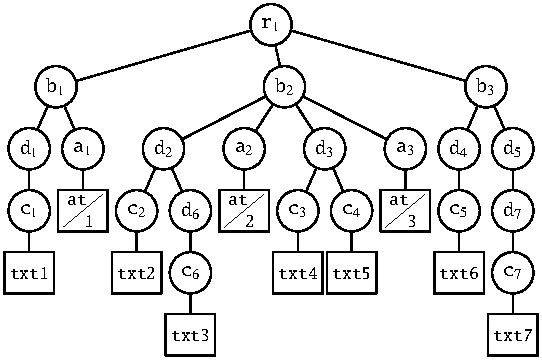
\includegraphics[scale=1.1]{partialtree/figures/bfstree.pdf}
	\caption{An example XML tree with values.}
    \label{fig:bfstree}
\end{figure}

\begin{figure}[t]
	\centering
	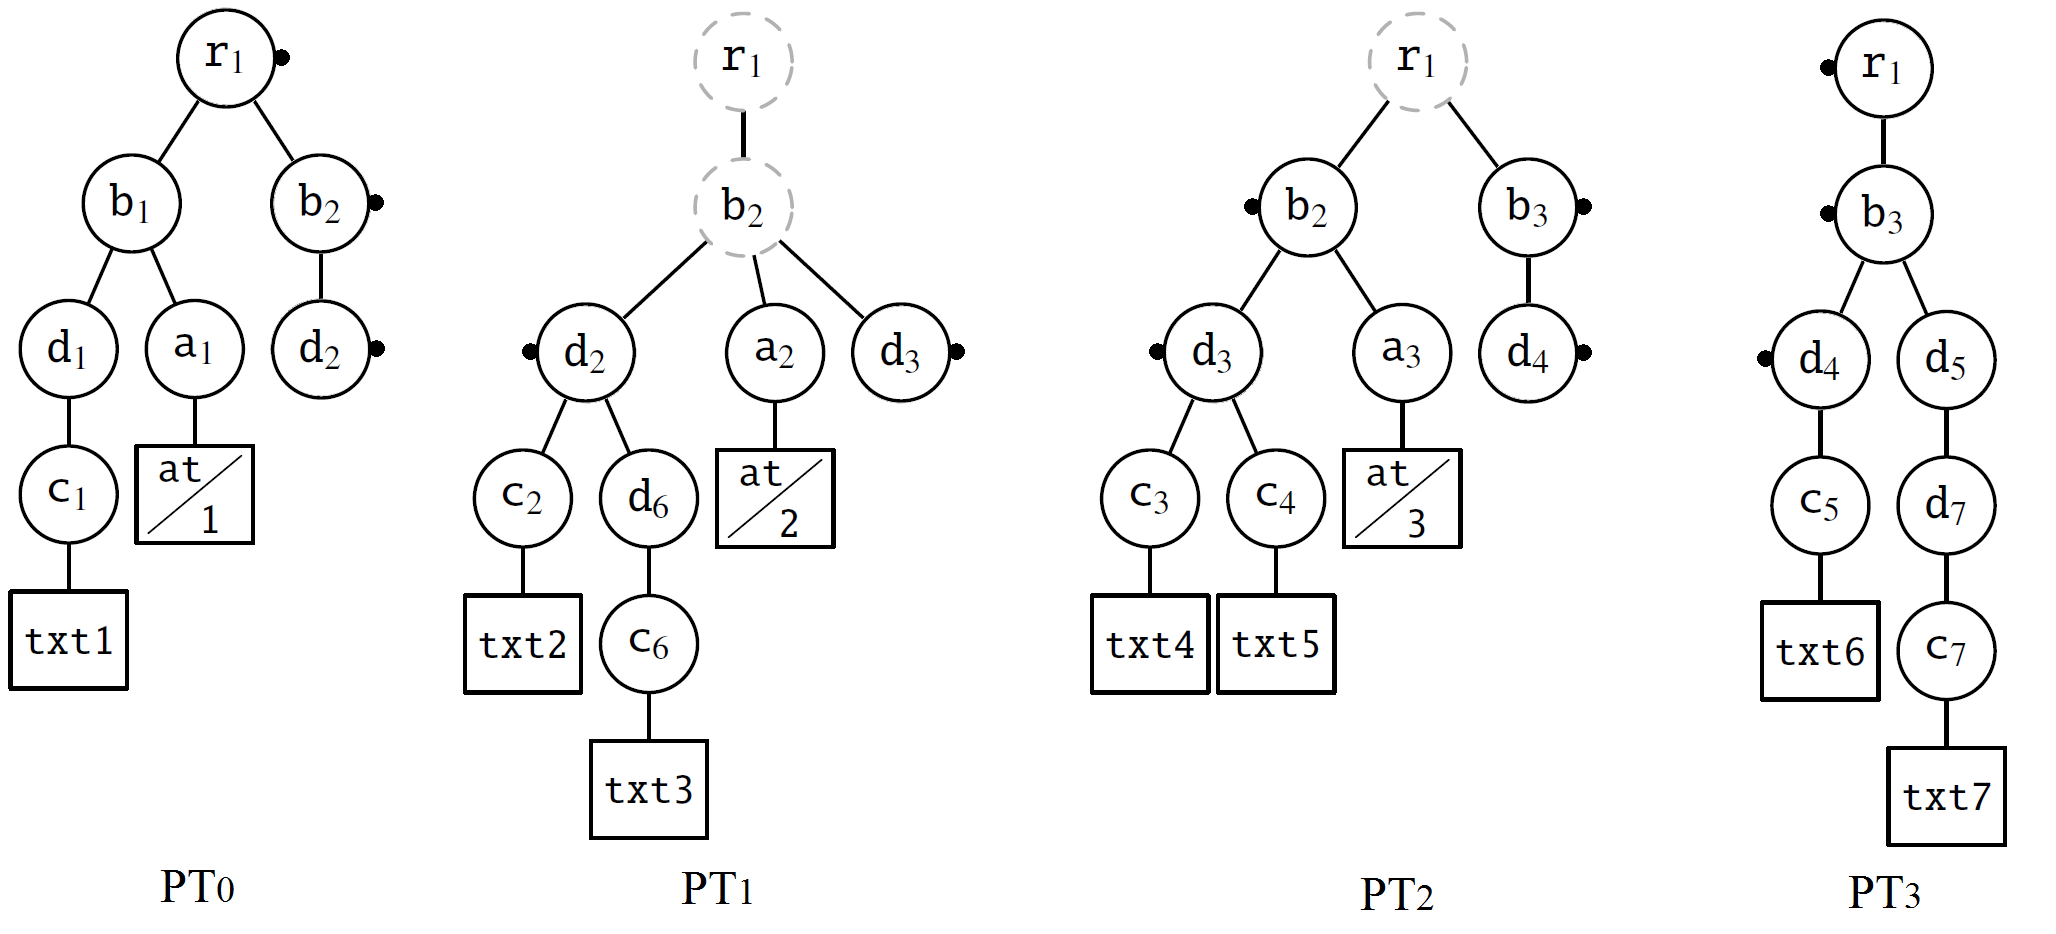
\includegraphics[scale=0.26]{partialtree/figures/bfstrees.png}
	\caption{Partial trees with values from the XML document.}
	\label{fig:bfspartialtree}
\end{figure}

For the four partial trees, we represent element nodes, attribute nodes and
value nodes consistent as the original XML tree. Since the partition only
affects the element node, from which the open nodes are only generated and
attribute nodes and content nodes can be simply implementated by the idea of
partial tree. As we have introduced in Section~\ref{sec:construction}, the split
tags are merged in case when the split position falls inside a tag and thus
splits the tag into two halves. In case of a text node is split into two sub
texts and separated on different partial trees, we simply merge the split two
sub texts into one and leave it on one partial tree. Thus this makes the
algorithm consistent.

The partial trees in the previous section provide a nice fragmentation of an XML
tree, making it possible for data parallel processing. To develop a
high-performance query framework, we still need to design concrete data
representation taking the following two issues into consideration.

\textbf{Expressiveness}

Originally indexing (or labeling) was considered to put shredded XML data into
databases~\cite{BGvM06,OOPC04}, but its expressiveness is very important to
accelerate queries.

\textbf{Compactness}

In the case we repeatedly apply several queries on the same data, we can put all
the indices in memory to avoid expensive I/O cost.

The first design choice is about the updates of XML data. In general purpose
framework, efficient support of updates is an important issues and several
frameworks support updates with sophisticated indexing such as
ORDPATH~\cite{OOPC04}. However, such an index with the update capability tends
to be large and complicated to handle. In this study, we decided not to allow
users to update XML data, which makes the implementation much simpler and
faster. We expect that users can fulfill their objective without updating the
XML data themselves,  if we provide some programming interface over the
framework.

The second design choice is about the functionality that the indices provide. An
important goal of this work is to support queries with not only the
\texttt{child} and \texttt{descendant} axes but also order-aware ones such as
\texttt{following-sibling} and \texttt{following}. To achieve our goal, the
following functions should be efficiently implemented.

\begin{figure*}[t]
	\centering
	\begin{minipage}{.2\linewidth}
		Partial tree\\[15pt]
		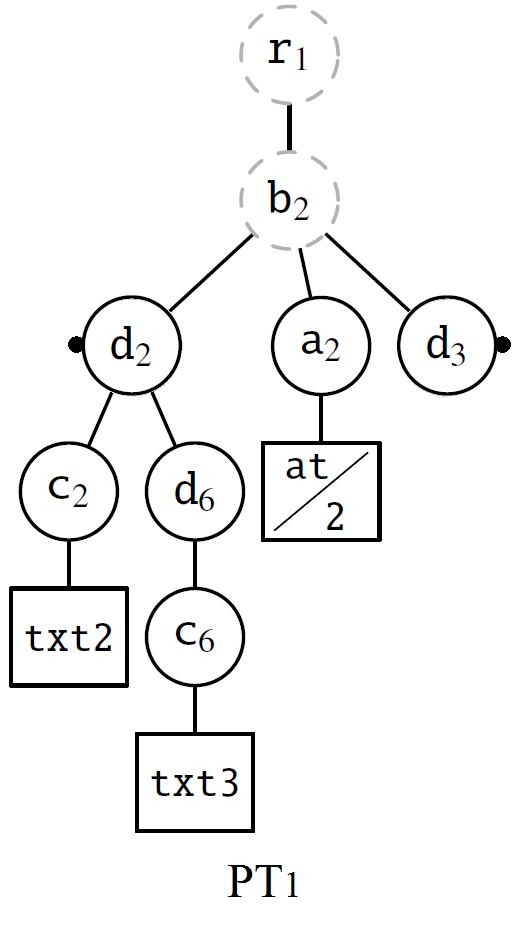
\includegraphics[scale=.25]{partialtree/figures/bfspt1.png}
	\end{minipage}
	\begin{minipage}{.55\linewidth}
		BFS-array \\
		\begin{tabular}{c|lcrrrr}
			\hline
			index   & tag             & type &  st & ed  & par    &  ch \\
			\hline
			1  & 5 (\texttt{r})  & N-OO &  0  & 196 &   0    &  2  \\
			2  & 2 (\texttt{b})  & N-OO & 42  & 142 &   1    &  3  \\
			3  & 4 (\texttt{d})  & N-OC & 45  &  81 &   2    &  6  \\
			4  & 1 (\texttt{a})  & N-CC & 81  &  95 &   2    &  8  \\
			5  & 4 (\texttt{d})  & N-CO & 95  & 124 &   2    &  9  \\
			6  & 3 (\texttt{c})  & N-CC & 48  &  59 &   3    &  9  \\
			7  & 4 (\texttt{d})  & N-CC & 59  &  77 &   3    & 10  \\
			8  & 6 (\texttt{at}) & A    & 88  &  88 &   4    & 11  \\
			9  & 0               & T    & 51  &  55 &   6    & 11  \\
			10 & 3 (\texttt{c})  & N-CC & 62  &  73 &   7    & 11  \\
			11 & 0               & T    & 65  &  69 &  10    & 12  \\
			\hline
		\end{tabular}
	\end{minipage}
    \begin{minipage} {.2\linewidth}
    Grouping Array \\[15pt]
 	\begin{tabular}{c|l}
 	\hline
 	tag  &   index      \\
 	\hline
 	0  &  $[9, 11]$ \\
 	1  &  $[4]$ \\
 	2  &  $[2]$ \\
 	3  &  $[6]$  \\
 	4  &  $[3,5,7]$  \\
 	5  &  $[1]$  \\
 	6  &  $[8]$  \\
 	\hline
    \end{tabular}
\end{minipage}
	\caption{A partial tree and its representation with two arrays}
	\label{fig:2arrays}
\end{figure*}

\begin{itemize}
	\item Function $\mathsf{getChildren}(x)$ returns all the children of node $x$.
	\item Function $\mathsf{getParent}(x)$ returns the parent of node $x$.
	\item Function $\mathsf{nextSibling}(x)$ returns the next (right) sibling of node $x$.
	\item Function $\mathsf{prevSibling}(x)$ returns the previous (left) sibling of node $x$.
	\item Function $\mathsf{isDescendant}(x, y)$ returns true if node $x$ is a descendant of node $y$.
	\item Function $\mathsf{isFollowing}(x, y)$ returns true if node $x$ is strictly after node $y$ in the document order.
	\item Function $\mathsf{getNodesIn}(t, x)$ returns all the nodes with tag $\mathit{t}$ in the subtree rooted at $x$.
\end{itemize}

We design two index sets (Fig.~\ref{fig:2arrays}) to provide these functions
keeping the indices compact. A node has the following fields:

\begin{itemize}
	\item $\mathit{tag}$: tag names (they are short integers that map to the strings),
	\item $\mathit{type}$: type of nodes including the four node types,
	\item $\mathit{st}$: start position (the position in the file to avoid global counting), and
	\item $\mathit{ed}$: end position.
\end{itemize}

The first index, \emph{BFS-array}, lists all the nodes in the order of the
breadth first search (BFS). Every node has two integer pointers to its parent
($par$) and the first child ($ch$) in this list. With the BFS order and these
two pointers, we can compute functions $\mathsf{getChildren}$,
$\mathsf{getParent}$, $\mathsf{nextSibling}$, and $\mathsf{prevSibling}$
efficiently. The second index, \emph{Grouped-array}, groups the nodes by their
tag names and then sorts the nodes in the groups by their start position.  With
this index, we can evaluate the function $\mathsf{getNodesIn}$ efficiently.

In our implementation, we used
2 bytes for $\mathit{tag}$,
1 bytes for $\mathit{type}$,
8 bytes for $\mathit{st}$,
8 bytes for $\mathit{ed}$,
4 bytes for $\mathit{par}$,
4 bytes for $\mathit{ch}$, and
4 bytes for $\mathit{idx}$.
(Though total file size could exceeds 32 bits, we assume that the number of
elements in a single partial tree can fit in 32 bits.) The total size needed for
representing a node is $2 + 1 + 8 + 8 + 4 + 4 + 4 = 31$ bytes, which is much
smaller than several implementation of DOM trees or databases. This is a key to
achieve high-performance evaluation of queries.


\section{Evaluation}
\label{sec:evaluation}

In this evaluation to our indexing, we conducted experiments for two aims: \\
1) to investigate the absolute query time with 100s GB of XML data.\\
2) to explore the scalability of our implementation on processing 
a large XML documents over a number of computing nodes.\\
We also compare ours with BaseX, the state-of-the-art XML database engine, in 
order to understand the performance of our indexing.

\subsection{Absolute Query Time} 

\subsubsection{Hardware Settings}

We used were Amazon Elastic Compute Cloud (EC2) M3 for this experiment. M3
Instances are general purpose compute instances that are powered by E5-2670 v2
(Ivy Bridge), equipped with 30 GB of memory and 2 X 80 GB of SSD, running Amazon
Linux AMI 2016.09.0. and offer a balance of compute, memory, and networking
resources for a broad range of workloads. We used m3.2xlarge instances for this
experiment, The network among EC2 instances was a local network and the network
speed is 1 gbps. The java running on m3.2xlarge was 64-Bit JVM (build
25.91-b14).


\subsubsection{Datasets and XPath Queries}

There were three datasets used in this experiment, the statistics of which are
shown in Table~\ref{tab:datasets}. For XMark datasets, we used the XML document
generator \emph{xmlgen} from XMark
project\footnote{\url{http://www.xml-benchmark.org/}}. The XMark xmlgen takes an
float number \emph{f} to determine the size of output dataset. 
For the experiments on a single EC2 instance,  we used two typical datsets: DBLP
and XMark~\cite{XMark} (with factor 100). For parallel processing, we used
XMark(with factor 2000) and UniProtKB. The UniProtKB dataset has a root element
with a large number of children with the same tag name and thus can be easily
well-formed  to be processed by multiple processors.  In contrast, XMark
datasets whose root has only six children  with different tag names, each
containing different amounts of data, makes it difficult to be well-formed.
Table 2 shows the 15 queries covering the three cases: XQ1 and UQ1 to test long
queries with nested predicates;  XQ2, DQ1, DQ2, UQ2, UQ4 and UQ5 to test
backward axes;  and the rest to test order-aware queries.

\begin{table}
	\small
	\caption{Statistics of XML dataset.}
	\label{tab:datasets}
	\begin{tabular}{c|c|c|c|c}
		\hline
		Datasets & dblp.xml & xm100.xml & xm2000.xml & uniprot.xml \\
		\hline \hline
		Nodes & 43,131,420 & 163,156,531 & 3,262,490,248 & 7,891,267,994 \\
		\hline
		Attributes & 10,885,411 & 42,257,706 & 845,072,591 & 9,254,412,578 \\
		\hline
		Values & 39,642,166 & 67,254,767 & 1,344,932,943 & 1,490,598,653 \\
		\hline
		Total & 93,658,997 & 272,669,004 & 5,452,495,782 & 18,636,279,225 \\
		\hline
		\# of tags & 47 & 77 & 77 & 82 \\
		\hline
		Size $($byte$)$ & 1,912,866,012 & 11,758,954,863 & 236,138,315,428 & 383,954,056,809 \\
		\hline
		Depth & 6 & 13 & 13 & 7 \\
		\hline
	\end{tabular}
	\vspace{10px}
	\caption{Queries used in the experiments.}
	\begin{tabular}{c|c|l}
		\hline \hline
		Name & Dataset & Query  \\
		\hline
		XQ1 & xmark & /site/closed\_auctions/closed\_auction[annotation/ \\
		&&description[text/keyword]]\\
		\hline
		XQ2 & xmark & /site//keyword/ancestor::mail \\
		\hline
		XQ3 & xmark & /site/open\_auctions/open\_auction  \\
		&&/bidder[1]/increase\\
		\hline
		XQ4 & xmark & /site/people/person/name/following-sibling::emailaddress \\
		\hline
		XQ5 & xmark & /site/open\_auctions/open\_auction[bidder\\
		&&/following-sibling::bidder]/reserve\\
		\hline
		DQ1 & dblp & /dblp//i/parent::title\\
		\hline
		DQ2 & dblp & //author/ancestor::article \\
		\hline
		DQ3 & dblp & /dblp//author/following-sibling::author \\
		\hline
		DQ4 & dblp & //author[following\textemdash sibling::author] \\
		\hline
		DQ5 & dblp & /dblp/article/title/sub/sup/i/following::author \\
		\hline
		UQ1 & uniprot & /entry[comment/text]/reference[citation \\
		&&/authorList[person]]//person\\
		\hline
		UQ2 & uniprot & /entry//fullName/parent::recommendedName \\
		\hline
		UQ3 & uniprot & /entry//fullName/following::gene \\
		\hline
		UQ4 & uniprot & //begin/ancestor::entry\\
		\hline
		UQ5 & uniprot & //begin/parent::location/parent::feature/parent::entry \\
		\hline
	\end{tabular}
\end{table}


\begin{table}[t]
	\centering
	\caption{Evaluation by one EC2 instance}
	\label{tab:singeval}
	\begin{tabular}{c|c|c|c|c|c|c|c|c|c|c}
		\hline \hline
		Dataset  & \multicolumn{5}{c|}{xmark10.xml} & \multicolumn{5}{c}{dblp.xml} \\ \hline
		Time     & \multicolumn{5}{c|}{8.5}          & \multicolumn{5}{c}{47}       \\ \hline
		Memory   & \multicolumn{5}{c|}{222}          & \multicolumn{5}{c}{3.1}       \\ \hline
		Query    & XQ1  & XQ2   & XQ3 & XQ4  & XQ5  & DQ1 & DQ2 & DQ3  & DQ4  & DQ5 \\ \hline
		Time(ms) & 591  & 1888  & 494 & 1771 & 1784 & 11  & 786 & 1863 & 3254 & 602 \\ \hline
	\end{tabular}
	\vspace{10px}
	\caption{Evaluation by multiple EC2 instance}
	\centering
	\label{tab:multieval}
	\begin{tabular}{c|c|c|c|c|c|c|c|c|c|c}
		\hline \hline
		Dataset	&	\multicolumn{5}{|c|}{xm2000.xml}     & \multicolumn{5}{c}{unirpot.xml}       \\
		\hline
		Loading (ms)	&	\multicolumn{5}{|c|}{210}     & \multicolumn{5}{c}{379}       \\
		\hline
		Memory (GB)	&	\multicolumn{5}{|c|}{173}     & \multicolumn{5}{c}{560}       \\
		\hline
		Query	& QX1      & XQ2     & QX3      & QX4      & QX5      & UX1      & UX2      & UX3      & UX4      & UX5      \\
		\hline
		Time Taken (ms) & 5951 & 819 & 1710 & 1168 & 3349 & 2573 & 2408 & 1324 & 5909 & 6220\\
		\hline
	\end{tabular}
\end{table} 

\subsection{Evaluate Queries on a Single EC2 Instance}

This experiment is to investigate the query performance on a single EC2
instance. In this case, we use the whole input XML document as a chunk and only
one partial tree generated from the chunk. Thus the queries are evaluated in
serial. The results show that for both datasets, it can process the queries
in 100s ms to several seconds. These reaults is helpful for us to understand
the query performance of partial tree in serial.


\subsection{Evaluate Queries on Multiple EC2 Instances}

In this experiment, we investigate the query performance processing 100s GB of
XML document on 32 EC2 instances. We use UniProtKB and XMark2000(f = 2000) as
experimental data. The results are shown in Table~\ref{tab:multieval}. 

In the parsing phase, for 0.545 billion and 1.86 billion elements, each of which
takes 31 bytes, the memory consumption should 157 GB and 537 GB respectively.
The experimental results show the memory consumption are 173 and 560 GB, which
are close to our analysis.  The overheads is some intermediate data generated
during construction. The parsing times as shown in Table 3 are relatively short
with regard to the data sizes. The evaluating results for XQ1 to XQ5 in Table~3
show that  the query times are just a few seconds for evaluating 220 GB and 358
GB XML data.  Besides, the loading times are just 210s and 379s.  The throughput
is around 1 GB/s. For comparison, PP-Transducer~\cite{OgTP13} achieved the best
throughput of 2.5 GB/s by using 64 cores. Although it is faster than ours, the
queries we can process are more expressive than PP-transducer, which does not
support order-aware queries.



\subsection{Scalability}
This experiment is used to explore the scalability of our indexing with up to 
64 workers.

\subsubsection{Dataset and XPath Queries} 

In our experiment, we set f to 160 and generated an 18.q54 GiB XML document
xmark160, which has 267 M element nodes, 61.3 M attribute nodes and 188 M
content nodes, totally 516.3 M nodes. We used 7 queries Q1 -- Q7 to evaluate our
implementation, including commonly used axes with predicate as  shown in
Table~\ref{tab:queries}.


\begin{table*}[ht]
	\centering
	\caption{Queries used for xmark160 dataset.}
	\label{tab:queries}
	\begin{tabular}{|l|l|l|}
		\hline
		querykey & query                                                                                  & hit nodes \\ \hline
		Q1       & /site/open\_auctions/open\_auction/bidder/increase                                     & 9577159   \\ \hline
		Q2       & /site//keyword                                                                         & 11271671  \\ \hline
		Q3       & /site//keyword/parent::text                                                            & 6503643   \\ \hline
		Q4       & /site//text{[}./keyword{]}                                                             & 6503643   \\ \hline
		Q5       & /site/people/person{[}./profile/gender{]}/name                                         & 1022629   \\ \hline
		Q6       & /site/people/person/name/following-sibling::emailaddress                               & 4080000   \\ \hline
		Q7       & /site/open\_auctions/open\_auction{[}./bidder/following-sibling::annotation{]}/reserve & 1734198   \\ \hline
	\end{tabular}
\end{table*}


\subsection{Hardware} 

The hardware we used were Amazon Elastic Compute Cloud (EC2) M5
Instances\footnote{\url{https://aws.amazon.com/ec2/instance-types/m5/}}. M5
Instances are general purpose compute instances that are powered by 2.5 GHz
Intel Xeon Scalable processors and offer a balance of compute, memory, and
networking resources for a broad range of workloads.  We used m5.2xlarge in our
experiment, which has 8 virtual cores, equipped with 32 GB of memory and
supported with solid state drives.  The instance runs Amazon Linux AMI 2018.03.0
(HVM) that supports Java by default. The Java version we used was "1.7.0\_181",
OpenJDK Runtime Environment (amzn-2.6.14.8.80.amzn1-x86\_64 u181-b00) OpenJDK
64-Bit Server VM (build 24.181-b00, mixed mode). The network among EC2 instances
was a local network and the network speed is 1 gbps.


\subsubsection{Running with a single worker}

The version of BaseX we used was 8.6.7 implemented on java 1.7. We ran it in
server/client mode. A BaseX server and a BaseX client were running on two EC2
instances. A database was created from xmark160 by the BaseX server. The server
was set in main memory mode and turned text indexing off for the creation to
make both BaseX and ours in the same setting.

To evaluate queries, we used the following XQuery expression for BaseX:  
\verb|for $node in db:open('xmark160')&query|\\
\verb|return db:node-pre($node)|, where  \verb|&query|
represents an XPath query. This expression returns a list of PRE-values and may
take a lot of time for sending and receiving among the BaseX server and a BaseX
client. Since network part is not what we are interested, we apply count() to
the results of the XPath query to both BaseX and ours so that the final outcome
will be only an integer to be returned over network, greatly removing the effect
of network.

As shown in Figure~\ref{fig:compare}, our indexing outperformances BaseX for all
the queries. Most of the queries takes only one half or one third time compared
with that of BaseX. The most significant one is Q2, for which ours is over 13
timers faster than BaseX. This is because in the two steps of Q2, \texttt{/site}
returns only 1 node, taking negligible time, while the second step,
\texttt{//keyword}, can greatly utilize the grouped-array to skip evaluating
most irrelevant nodes with different tag names as \texttt{keyword}, thus
achieving the best performance.


\begin{figure}[thb]
	\centering
	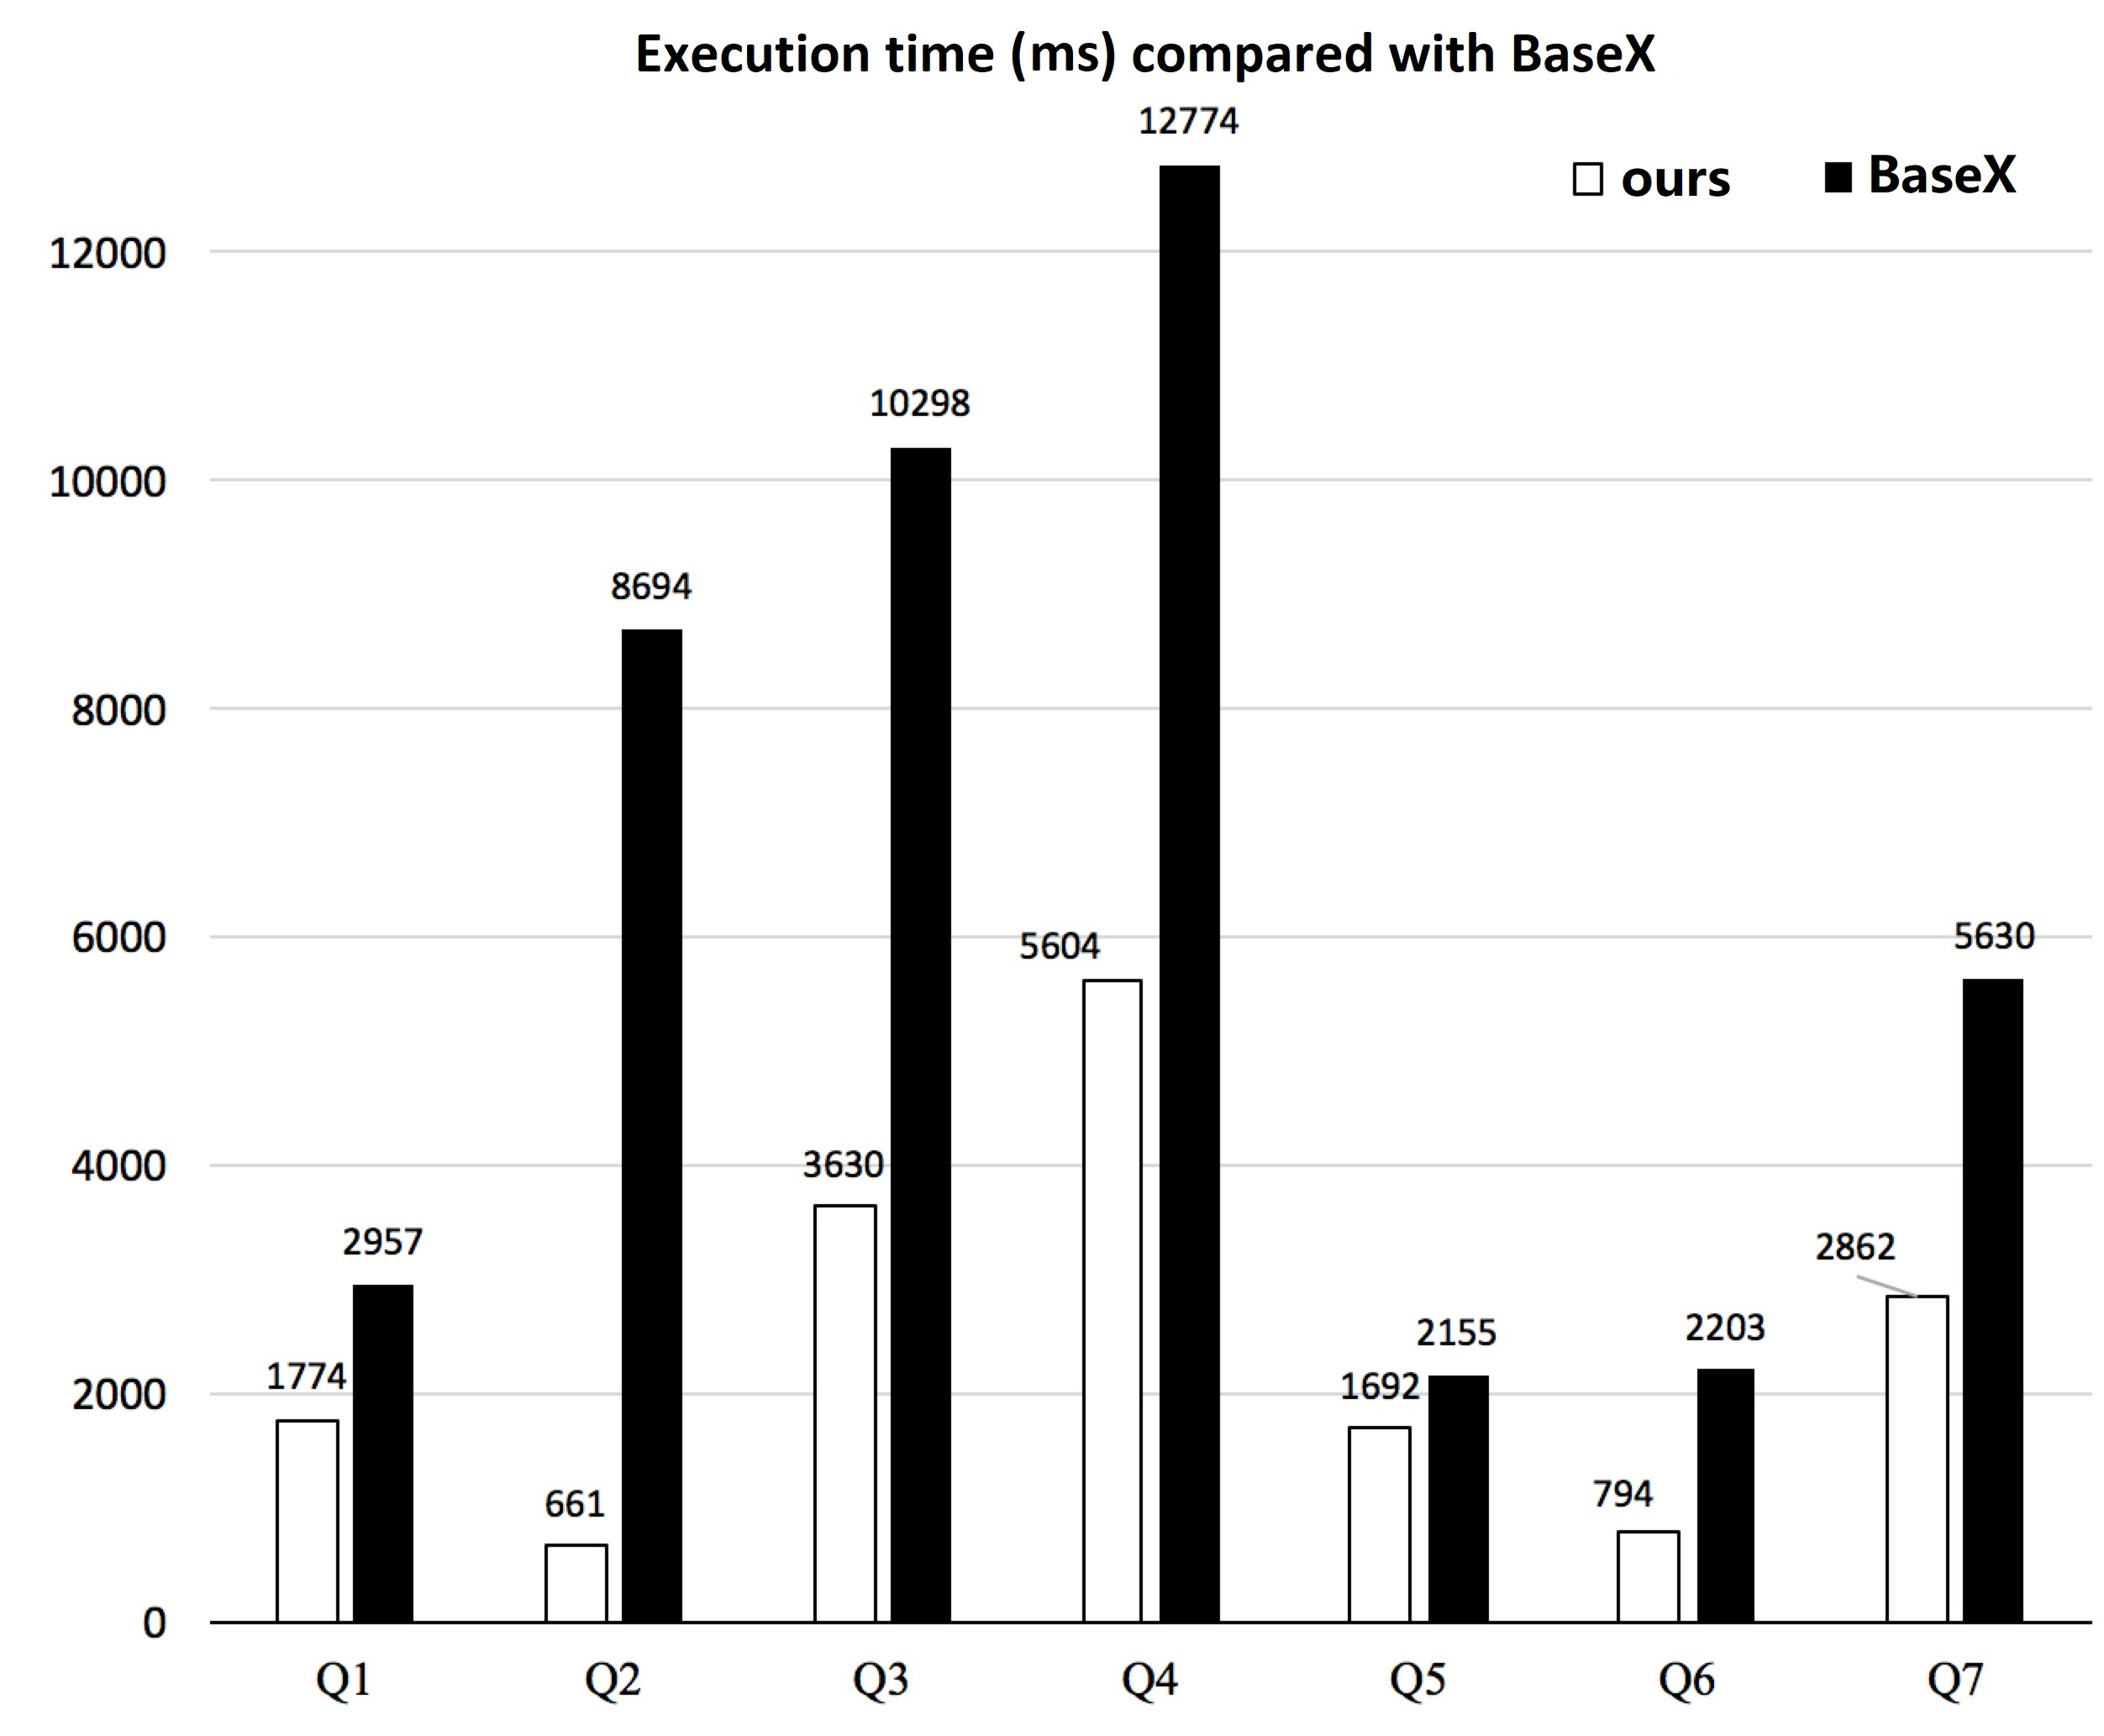
\includegraphics[width=0.9\linewidth]{compare}
	% figure caption is below the figure
	\label{fig:compare}       % Give a unique label
	\caption{Execution time (ms) compared with BaseX.}
\end{figure}

\begin{figure}[thb]
	\centering
	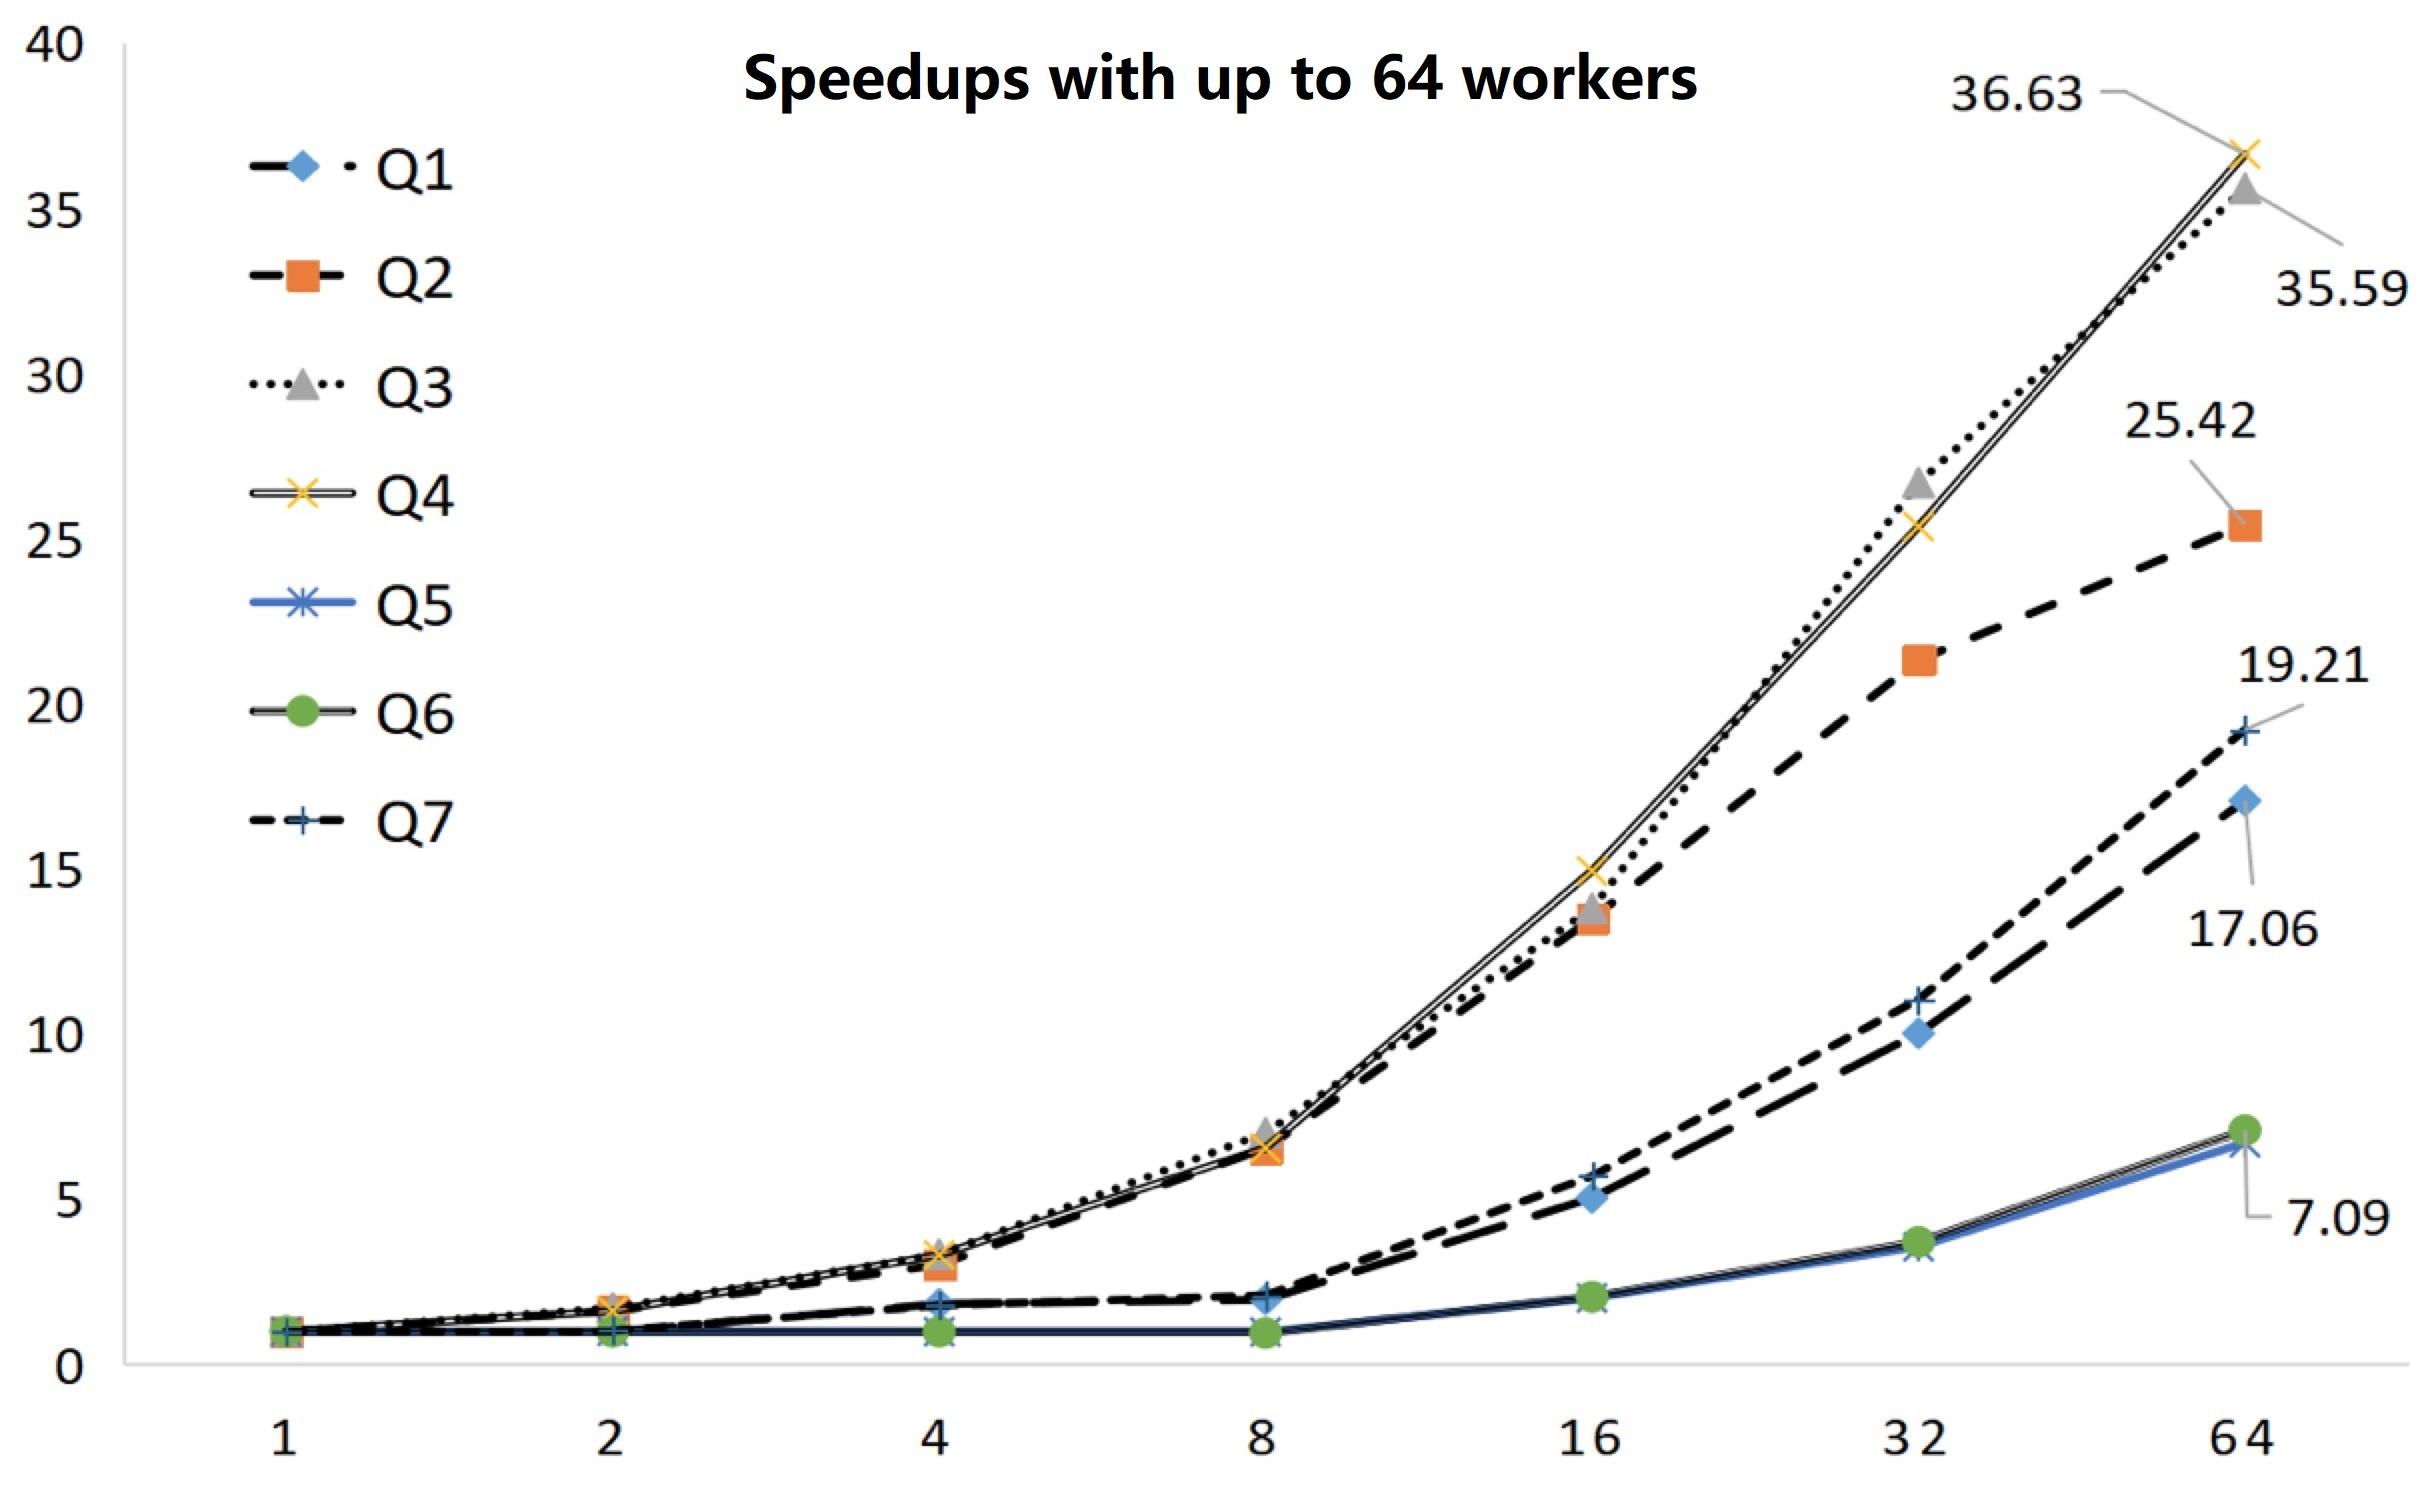
\includegraphics[width=0.9\linewidth]{speedups}
	\caption{Speedups with up to 64 workers.}
	\label{fig:speedups}    
\end{figure}


\subsubsection{Processing Queries in Parallel With Mutiple Workers}

This experiment is to test the speedups using our indexing on multiple EC2
instances. In this experiment, we use 1 instance for the master to control
query processing and 8 instances for workers to execute queries. Since the
instance m5.2xlarge has 8 cores, we arranged at most 8 workers on a single
instance. Given 8 instances, there are totally 64 workers involved in the
computation, as well as 64 chunks we divided at most. Due to the imbalance of
xmark160, not all the worker may have hit nodes of running queries. Thus, we
call workers that have hit nodes active workers, while for the rest idle
worker. 

The XML dataset xmark160 is divided into different number of chunks, to be
processed by different numbers of workers on up to 8 instances. From each chunk,
a partial tree will be created. It will be possessed and processed by a single
worker (we assign only one chunk to a worker in this experiment). 

To achieve better load balance, we used cyclic distribution to assign chunks to
instances. This means that we assign chunks to each instance, making consecutive
chunks be assigned to different instances. For example, given 8 chunks, $chunk_1$,
$chunk_2$, ..., $chunk_9$,  and 4 computing nodes, $com_1$, $com_2$, ..., $com_4$, 
we assign them as 
$com_1$($chunk_1$, $chunk_5$), 
$com_2$($chunk_2$, $chunk_6$), 
$com_3$($chunk_3$, $chunk_7$), 
$com_4$($chunk_4$, $chunk_8$). 
In such order, we can make the workers utilize the resources of computing nodes. 

We record the wall-clock time form the master's side. The timing starts from the
master sending a message to all workers to start a query, and ends at the moment
when the master receives the work-done message from the last worker, denoting
querying work is complete. The execution times are listed in
Table~\ref{tab:exetimes}.


\begin{table*}[ht]
	\centering
	\caption{Execution time in milliseconds).}
	\label{tab:exetimes}
	\begin{tabular}{|c|c|c|c|c|c|c|c|}
		\hline
		\# of workers & 1       & 2       & 4       & 8       & 16      & 32      & 64      \\ \hline
		Q1                & 1774    & 1789    & 968     & 905     & 352     & 177     & 104 \\ \hline
		Q2                & 661     & 410     & 219     & 101     &  49     & 31      & 26 \\ \hline
		Q3                & 3630    & 2120    & 1090    & 518     & 263     & 136     & 102 \\ \hline
		Q4                & 5604    & 3467    & 1695    & 855     & 375     & 221     & 153 \\ \hline
		Q5                & 1692    & 1685    & 1709    & 1731    & 841     & 475     & 252 \\ \hline
		Q6                & 794     & 800     & 803     & 834     & 388     & 214     & 112 \\ \hline
		Q7                & 2862    & 2817    & 1595    & 1369    & 502     & 259     & 149 \\ \hline
	\end{tabular}
\end{table*}

From the results, we have the following observations.

\subsubsection{Execution Time Reduced with More Workers}

From the results in the table, it is clear that with the number of workers
increased, the execution times of most queries are reduced. For
example, the execution time is nearly halves every time when the number of
workers doubled for Q3. It clearly showed that the parallel processing of
XPath queries using our index is efficient to reduce execution time by using 
more workers.

\subsubsection{Imbalance of XML Document Can Prevent Speedups}

As we can also notice, however, there are some cases execution times do not
reduce at all even with more workers. For example, no matter the number of
workers increased is 1, 2, 8 or 8, the execution times of all the cases are
still basically the same.  We analyzed the number of active workers and found
that this is caused by the imbalance of XMark datasets. In the xmark160, the hit
nodes of queries may only reside on a consecutive part of the XML document.
Then, after being divided, the hit nodes may be distributed in a small number of
chunks. Thus, only the workers that possess these chunks can be active, while
the rest workers just stay idle. Let us continue to take Q5 as an example. When
the number of workers increases from 1 to 8, the number of active nodes,
however, does not increase and still stays 1, i.e. there was only one active
worker for the query. Therefore, with only one worker, it takes nearly the same
amount of time to process the same amount of hit nodes regardless how many
workers were totally used. 

\subsubsection{Imbalance of XML Document Can Spoil Speedups}

We also notice that some execution times are not reduced much when even when
more active workers involve. For example, Q2 takes 661 ms by one active worker
and 410 ms for two active workers, the execution is not halved. This is because
the hit nodes did not evenly distributed over the two active workers. As we
investigated, one worker took 406 ms to collect 6785094 hit nodes, while another
worker took 256 ms for 4486577 hit nodes. Therefore, the speedup is degraded due
to the imbalanced distribution of hit nodes over chunks. We can learn that the
imbalance can not only prevent the speedup, but also can degrade the speedup.

To understand how much speedup ours can achieve, we use the execution time done
by a single worker as baseline. The results are shown in
Figure~\ref{fig:speedups}.  From the figure, it shows that ours can achieve
better speedup when using more workers. The best speed up is done from Q3 by a
factor of 36.63. We also notice that when the number of workers are large than
8, the speedup becomes dramatical, which means with more chunks divided, the
imbalance can be smoothed and it can be more effective for better speedups. This
is because  with smaller chunks, hit nodes can be distributed to more chunks;
meanwhile,  with the cyclic distribution of these small chunks, we can have more
active workers to participate in the querying process, thus achieving better
speedups. 


\subsubsection{Discussion}

From the experiment results and our analysis in previous sub section, we suggest
that it is better to assign more chunks to a worker rather than one as what we
conducted in the experiment. In such case, more workers will possess chunks that
contain hit nodes. In ideal case, hit nodes consecutively contained in a part of
the XML document can be divided into more chunks, and these chunks can be
distributed to each of workers.  Then, all the workers become active and we can
achieve better speedups. However, with too many chunks, it is not clear how
much overhead on memory, thread or network etc will be involved. We need to find
a trade-off about the maxamum number of chunks to reach the best performance.
Thus, it is worth studying for the future work.



 

%\section{Summary}

In this chapter, we have first developed a novel tree structure called partial
tree based on a vertical fragmentation of XML documents. To construct partial
trees from an XML document, there are four phases. First, we split the XML
document into several chunks. Second, we parse the chunks in parallel to form
several sets of subtrees that have some open nodes. Third, we compute pre-paths
from all open nodes. Last, we put pre-paths to each corresponding set of
subtrees to complete the partial tree construction.

After the introduction to partial tree, we have also designed query algorithms
for most useful class of XPath queries with three examples to demonstrate how
the query algorithms work.

Last, we have implemented partial tree with a BFS-array based index for high-
efficiency. The experiment shows that the implementation reaches a good absolute
query time that can evaluate XPath queries over 100s GB of XML documents in 100s
millisecond to several seconds.



% In this paper, we use the same set of queries over
% XMark\footnote{\url{http://www.xml-benchmark.org/generator.html}}
% \cite{schmidt02:xmark} datasets as \cite{BoLS09}.  Table~\ref{tbl:query}
% summarizes our target queries, where (a)--(c) mean variations of data
% partitioning and (a)--(b) except for XM6(b) follow ones used in \cite{BoLS09}.


\bibliographystyle{ieeetr} % Title is link if provided
\bibliography{backmatter/references} % adjust this to fit your BibTex file




\end{document}
